\documentclass[a4paper,11pt]{book}
%\documentclass[a4paper,twoside,11pt,titlepage]{book}
\usepackage{listings}
\usepackage[utf8]{inputenc}
\usepackage[spanish,es-tabla]{babel}

% \usepackage[style=list, number=none]{glossary} %
%\usepackage{titlesec}
%\usepackage{pailatino}

%\decimalpoint
\usepackage{dcolumn}
\usepackage{float}
\newcolumntype{.}{D{.}{\esperiod}{-1}}
\makeatletter
%\addto\shorthandsspanish{\let\esperiod\es@period@code}
\makeatother


%\usepackage[chapter]{algorithm}
\RequirePackage{verbatim}
%\RequirePackage[Glenn]{fncychap}
\usepackage{fancyhdr}
\usepackage{graphicx}
\usepackage{afterpage}
\usepackage[a4paper]{geometry}

\usepackage{longtable}

\usepackage[pdfborder={000}]{hyperref} %referencia

% ********************************************************************
% Re-usable information
% ********************************************************************
\newcommand{\mySubject}{Trabajo Fin de Grado\xspace}
\newcommand{\myTitle}{Desarrollo de Módulos de Visualización para Sistema de Recuperación de Imágenes\xspace}
\newcommand{\myEngTitle}{Visualization Module Development for Image Retrieval System}
\newcommand{\mySubTitle}{Módulos para visualizar el resultado obtenido por un sistema de recuperación de imágenes 
mediante el uso de un entorno 3d interactivo}
\newcommand{\myEngSubTitle}{Modules to display the result obtained by a image retrieval system
using an 3d interactive environment}

\newcommand{\myDegree}{Grado en Ingeniería informática\xspace}
\newcommand{\myName}{Alejandro Casado Quijada\xspace}
\newcommand{\myProf}{Jesús Chamorro Martínez\xspace}
\newcommand{\myEmail}{alex22alex33@correo.ugr.es\xspace}
%\newcommand{\myOtherProf}{Nombre Apllido1 Apellido2 (tutor2)\xspace}
%\newcommand{\mySupervisor}{Put name here\xspace}
\newcommand{\myFaculty}{Escuela Técnica Superior de Ingenierías Informática y de
Telecomunicación\xspace}
\newcommand{\myFacultyShort}{E.T.S. de Ingenierías Informática y de
Telecomunicación\xspace}
\newcommand{\myDepartment}{Departamento de Ciencias de la Computación e Inteligencia Artificial \xspace}
\newcommand{\myUni}{\protect{Universidad de Granada}\xspace}
\newcommand{\myLocation}{Granada\xspace}
\newcommand{\myTime}{\today\xspace}
\newcommand{\myVersion}{Version 0.1\xspace}
\renewcommand{\chaptername}{Capítulo}

\hypersetup{
pdfauthor = {\myName \myEmail},
pdftitle = {\myTitle},
pdfsubject = {\myTitle},
pdfkeywords = {image visualization, java 3D, image retrival, 3d visualization},
pdfcreator = {LaTeX con el paquete gedit},
pdfproducer = {pdflatex}
}

%\hyphenation{}


%\usepackage{doxygen/doxygen}
%\usepackage{pdfpages}
\usepackage{url}
\usepackage{colortbl,longtable}
\usepackage[stable]{footmisc}
%\usepackage{index}

%\makeindex
%\usepackage[style=long, cols=2,border=plain,toc=true,number=none]{glossary}
% \makeglossary

% Definición de comandos que me son tiles:
%\renewcommand{\indexname}{Índice alfabético}
%\renewcommand{\glossaryname}{Glosario}

\pagestyle{fancy}
\fancyhf{}
\fancyhead[LO]{\leftmark}
\fancyhead[RE]{\rightmark}
\fancyhead[RO,LE]{\textbf{\thepage}}
\renewcommand{\chaptermark}[1]{\markboth{\textbf{#1}}{}}
\renewcommand{\sectionmark}[1]{\markright{\textbf{\thesection. #1}}}

\setlength{\headheight}{1.5\headheight}

\newcommand{\HRule}{\rule{\linewidth}{0.5mm}}
%Definimos los tipos teorema, ejemplo y definición podremos usar estos tipos
%simplemente poniendo \begin{teorema} \end{teorema} ...
\newtheorem{teorema}{Teorema}[chapter]
\newtheorem{ejemplo}{Ejemplo}[chapter]
\newtheorem{definicion}{Definición}[chapter]

\definecolor{gray97}{gray}{.97}
\definecolor{gray75}{gray}{.75}
\definecolor{gray45}{gray}{.45}
\definecolor{gray30}{gray}{.94}

\lstset{ frame=Ltb,
     framerule=0.5pt,
     aboveskip=0.5cm,
     framextopmargin=3pt,
     framexbottommargin=3pt,
     framexleftmargin=0.1cm,
     framesep=0pt,
     rulesep=.4pt,
     backgroundcolor=\color{gray97},
     rulesepcolor=\color{black},
     %
     stringstyle=\ttfamily,
     showstringspaces = false,
     basicstyle=\scriptsize\ttfamily,
     commentstyle=\color{gray45},
     keywordstyle=\bfseries,
     %
     numbers=left,
     numbersep=6pt,
     numberstyle=\tiny,
     numberfirstline = false,
     breaklines=true,
   }

% minimizar fragmentado de listados
\lstnewenvironment{listing}[1][]
   {\lstset{#1}\pagebreak[0]}{\pagebreak[0]}

\lstdefinestyle{CodigoC}
   {
	basicstyle=\scriptsize,
	frame=single,
	language=C,
	numbers=left
   }
\lstdefinestyle{CodigoC++}
   {
	basicstyle=\small,
	frame=single,
	backgroundcolor=\color{gray30},
	language=C++,
	numbers=left
   }


\lstdefinestyle{Consola}
   {basicstyle=\scriptsize\bf\ttfamily,
    backgroundcolor=\color{gray30},
    frame=single,
    numbers=none
   }


\newcommand{\bigrule}{\titlerule[0.5mm]}


%Para conseguir que en las páginas en blanco no ponga cabecerass
\makeatletter
\def\clearpage{%
  \ifvmode
    \ifnum \@dbltopnum =\m@ne
      \ifdim \pagetotal <\topskip
        \hbox{}
      \fi
    \fi
  \fi
  \newpage
  \thispagestyle{empty}
  \write\m@ne{}
  \vbox{}
  \penalty -\@Mi
}
\makeatother

\usepackage{pdfpages}
\raggedbottom
\begin{document}
\begin{titlepage}
 
 
\newlength{\centeroffset}
\setlength{\centeroffset}{-0.5\oddsidemargin}
\addtolength{\centeroffset}{0.5\evensidemargin}

\noindent\hspace*{\centeroffset}\begin{minipage}{\textwidth}

\centering

\includegraphics[width=0.9\textwidth]{imagenes/logo_ugr.jpg}\\[1.4cm]

\textsc{ \Large TRABAJO FIN DE MÁSTER\\[0.2cm]}
\textsc{ MÁSTER EN INGENIERÍA INFORMÁTICA}\\[1cm]
% Upper part of the page
% 
% Title
{\Huge\scalebox{.2}\bfseries Desarrollo de un Sistema de Recuperación de Imágenes para Plataformas Móviles
\\
}
\noindent\rule[-1ex]{\textwidth}{3pt}\\[3.5ex]

\end{minipage}

\vspace{2.5cm}
\noindent\hspace*{\centeroffset}\begin{minipage}{\textwidth}
\centering

\textbf{Autor}\\ {\myName}\\[2.5ex]
\textbf{Director}\\
{\myProf}\\[2cm]

\includegraphics[width=0.3\textwidth]{imagenes/etsiit_logo.png}\\[0.1cm]
\textsc{Escuela Técnica Superior de Ingenierías Informática y de Telecomunicación}\\
\textsc{---}\\
%\myLocation, \myTime\\
\end{minipage}
%\addtolength{\textwidth}{\centeroffset}
%\vspace{\stretch{2}}
\end{titlepage}



%\frontmatter
\renewcommand\contentsname{Contenido}
\tableofcontents

\renewcommand\listfigurename{Lista de Figuras}
\listoffigures

\renewcommand\listtablename{Lista de Tablas}
\listoftables


%\listoftables

%
%\mainmatter
%\setlength{\parskip}{5pt}

\chapter{Resumen}
\label{cap:resumen}

Este proyecto busca permitir al usuario realizar consultar a un sistema de recuperación de imágenes, visualizando las imágenes resultantes de dichas consultas de una manera atractiva, interactiva y amigable. En esta ocasión dicho sistema ha sido desarrollado para plataformas móviles, concretamente \textit{Android}.\\

Cuando hablamos de un sistema de recuperación de información, \textit{CBIR}, nos referimos a los sistemas basados fundamentalmente en descriptores de bajo nivel (color, textura, etc.) obtenidos directamente a partir de la imagen. En ellos la idea es, mediante una imagen consulta, comprobar como de parecidas son el resto, imágenes resultado, y presentar los resultados\\

Al tratarse de una plataforma móvil hay que tener muy en cuenta los recursos que va a requerir dicho sistema, por lo que hay que esta especialmente atentos a ellos, ya que si el sistema necesita demasiados recursos puede funcionar incorrectamente y provocar incluso malfunciomaniento del propio teléfono.\\

Se busca interactividad por parte del usuario, por ello será capaz de moverse a través de las imágenes, tanto consulta como resultado, realizando movimientos de \textit{scroll}. A su vez, se ha añadido mecanismos de ayuda, para que el usuario sepa en cada momento en que lugar se encuentra, ya que el resultado de una consulta puede ser de cientos de imágenes. Por otro lado, será capaz de modificar ciertos parámetros, como descriptor asociado, número de imágenes, para adecuar el uso del sistema a su experiencia deseada.\\

Todo lo descrito se va a desarrollar a partir de un CBIR concreto, Java Multimedia Retrieval©.\\ 

Para realizar la planificación se realizaron una serie de reuniones iniciales con mi tutor en las cuales se acordaron los objetivos y elementos que debía de tener este proyecto. Estos objetivos se dividieron entre una serie de semanas. Pero en todo momento sabía lo que debía de realizar. Por lo que cada pocas semanas realizábamos reuniones para comprobar si dichos objetivos acordados y planificados se cumplían, a su vez discutíamos detalles secundarios del proyecto, como leves mejoras en la interfaz.\\

Para llevar a cabo la planificación se ha usado la herramienta conocida como diagramas de Gantt, en el que se especifican los objetivos a cumplir en un periodo concreto de tiempo. Este diagrama se detallará más adelante en su correspondiente sección.\\

Para la realización de este proyecto se partía de una situación que podría considerarse prácticamente desde 0, debido a que no hay muchos proyectos relacionados. También hay que tener en mente el problema de lidiar con una plataforma móvil, ya que sus recursos son limitados y no tan potentes como los de un computador. A su vez, hay que cuidar el tiempo de ejecución de las consultas, pues si es demasiado elevado, provocaría que el usuario dejara de usar la aplicación.\\

Teniendo en cuenta lo descrito anteriormente, el resultado del proyecto ha sido satisfactorio. La aplicación resultante nos permite realizar consultas sobre las imágenes del teléfono, pudiendo elegir la imagen consulta desde la galería o desde la cámara del propio teléfono. Los tiempos de cálculo de consulta son más que aceptables, teniendo en cuenta que tras un primera consulta, se almacenan los resultados en una pequeña base datos, esto se detallará detalladamente más adelante. Por otro lado, el usuario puede editar ciertos parámetros de la consulta, lo que hace que la aplicación sea ajustable a las necesidades del usuario en cualquier momento.\\

Mencionar brevemente, que las conclusiones del trabajado han sido satisfactorias. El proyecto se ha llevado a cabo correctamente, cumpliendo todos los objetivos establecidos, se ha cubierto un hueco de mercado que estaba prácticamente vacío, los \textit{CBIR} para \textit{Android}, son puramente académicos y sus interfaces son demasiado simples.\\

A su vez, se especifican dos posibles trabajos futuros:

\begin{itemize}

\item Trabajar con código nativo usando \textit{Android ndk}

\item Mostrar estadísticas apoyándose en conjuntos difusos.

\end{itemize}


Esta memoria se encuentra bajo la licencia \textbf{Creative Commons Attribution-NonCommercial 4.0 International}, mientras que el código del proyecto se encuentra con licencia \textbf{GNU General Public License v3.0}\\

Todo el código así como una copia de esta memoria se puede encontrar en el repositorio del proyecto. \textbf{https://github.com/acasadoquijada/jmr-android}



%
\chapter{Introducción}
\label{cap:introduccion}

\section{Contextualización}

Debido al avance de la tecnologı́a, cada vez disponemos de más dispositivos con la capacidad de capturar imágenes. Esto ha provocado un importante incremento en las bases de datos de imágenes, lo que a su vez ha propiciado la aparición de metodologı́as para solventar el problema de la manipulación, gestión y recuperación de dicha información. En este caso cuando hablamos de metodologı́as nos referimos a los sistemas de recuperación de información, basados fundamentalmente en descriptores de bajo nivel (color, textura, etc.) obtenidos directamente a partir de la imagen. Estos sistemas se denominan CBIR.\\

La recuperación de información es la actividad de obtener recursos de información relevantes para una necesidad de información a partir de una colección de recursos de información. Las búsquedas pueden ser basadas en texto, o en otro tipo de indexación basada en contenido. Para realizar esta actividad se utilizan los sistemas de recuperación de información, que se encargan de gestionar todo lo necesario.\\

Un proceso de recuperación de información comienza cuando un usuario realiza una consulta al sistema. Estas consultas son declaraciones de necesidad de información, por ejemplo, buscar una frase en un motor de búsqueda. Las consultas no identifican a un único objeto de la base de datos o colección, si no que afecta a varios con distintos grados de relevancia.\\

Un objeto, en este ámbito, es una entidad que representa la información en una colección o base de datos. Sin embargo, al contrario de lo que pasaría en una consulta a un sistema clásico SQL, los resultados son clasificados. Esta clasificación es la principal diferencia respecto a las búsquedas en bases de datos tradicionales.\\

Hay que tener en cuenta que dependiendo de la aplicación, los objetos pueden ser textos, imágenes, audio o vídeos, por ejemplo. La mayoría de los sistemas de recuperación de información manejan una puntuación numérico sobre como coincide cada objeto de la base de datos con el objeto consulta, y ordena los objetos acorde a este valor numérico. Los que se encuentran en las primeras posiciones del ranking se muestran al usuario.\\

Para realizar las consultas, los sistemas de recuperación utilizan los denominados descriptores. Estos describen las características de los objetos que se encuentran en la colección de objetos accesibles por el sistema. Dado que en este trabajo nos vamos a centrar en un sistema de recuperación de información, vamos a hablar sobre sus múltiples descriptores, denominados descriptores visuales.\\

Estos descriptores representan características visuales de los objetos, siendo estos vídeos o imágenes. Describen características elementales como la forma, el color, o la textura, entre otros muchos.\\

Los descriptores visuales se encuentran divididos en dos grandes grupos:

\begin{itemize}

\item \textbf{Descriptores de información general}. Proporcionan descripciones sobre el color, formas, regiones y texturas.

\item \textbf{Descriptores de información de dominio específico}. Proporcionan información sobre sucesos que van apareciendo en escena. El reconocimiento de caras sería un ejemplo delimitado de este tipo.

\end{itemize}

\subsection{Descriptores de información general}

Como se ha mencionado, estos descriptores se encargan de representar distintas propiedades visuales elementales, como el color y la textura.

\subsubsection{Color}

Puede ser considerada como el atributo elemental del contenido visual. A continuación se especifican cinco formas para describir el color. Las tres primeras simbolizan la distribución del color. Las otras dos describen la distribución espacial del color y la relación del color en un conjunto o secuencia de imágenes.

\begin{itemize}
\item Dominant Color Descriptor (DCD)
\item Scalable Color Descriptor (SCD)
\item Color Structure Descriptor (CSD)
\item Color Layout Descriptor (CLD)
\item Group of frame (GoF) o Group-of-pictures (GoP)
\end{itemize}

\subsubsection{Textura}

Esta propiedad se encuentra desarrollada para caracterizar las regiones, o texturas de una imagen. Esto se lleva a cabo teniendo en cuenta la homogeneidad de las regiones y los histogramas de los bordes de esas regiones. Como representantes de este conjunto tenemos:

\begin{itemize}
\item Homogeneous Texture Descriptor (HTD)
\item Texture Browsing Descriptor (TBD)
\item Edge Histogram Descriptor (EHD)
\end{itemize}

\subsubsection{Forma}

En esta ocasión, estamos hablando de información semántica de gran relevancia, ya que los objetos son reconocidos visualmente por los seres humanos. La única manera de obtener dicha información es mediante la segmentación de la imagen. Desafortunadamente, aún no se encuentra completamente disponible, pero si disponemos de una serie de algoritmos que nos ofrecen buenas aproximaciones. Estos descriptores detallan formas, regiones y contornos, si hablamos de imágenes 2D, y volúmenes en el caso de 3D. Estos descriptores son:

\begin{itemize}
\item Region-based Shape Descriptor (RSD)
\item Contour-based Shape Descriptor (CSD)
\item 3-D Shape Descriptor (3-D SD)
\end{itemize}

 
Como se ha mencionado anteriormente, nos vamos a centrar en los sistemas de recuperación de imágenes, por lo que vamos a ver una serie de ejemplos sobre ellos.

\subsection{CBMIR}

Este CBIR es usado en ámbitos médicos, de ahí su nombre Content-based medical image retrieval, ha sido desarrollado por la universidad nacional de Malasia. Se centra en ayudar a diagnosticar irregularidades vertebrales, lo cual es muy importante si se realiza a tiempo para disminuir el riesgo de sufrir fracturas vertebrales. Las fracturas aparecen en radiografías, pero su detección es poco frecuente por parte de médicos y radiólogos. Por esta razón, el objetivo de este CBIR es ayudar al personal sanitario a detectar estas irregularidades como se ha comentado anteriormente.\\

Una vez definido este CBIR, veamos como visualiza la información de una consulta.\\

\begin{figure}[H] %con el [H] le obligamos a situar aquí la figura
\centering
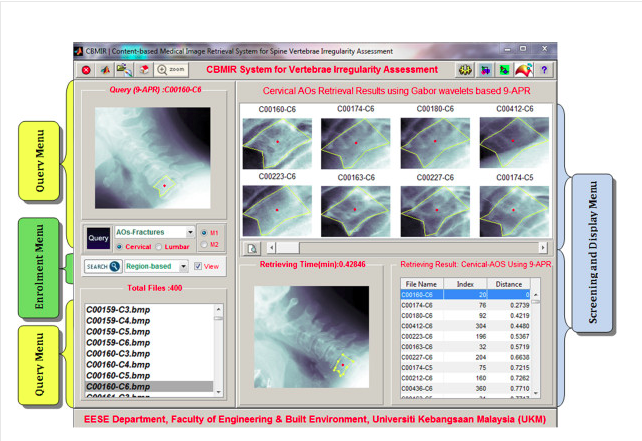
\includegraphics[scale=0.5]{imagenes/CBMIR.png}  %el parámetro scale permite agrandar o achicar la imagen. En el nombre de archivo puede especificar directorios
\label{CBMIR}
\caption{Sistema de recuperación de imágenes CBMIR}
\end{figure}

La visualización se realiza en la parte derecha de la pantalla. En la parte superior se aprecian todas las imágenes resultantes de la consulta, mientras que en la parte inferior podemos obtener mas información sobre cada una de esas imágenes.\\

Mientras que para la consulta se utiliza la parte izquierda. En ella se puede seleccionar el descriptor y la imagen a usar.\\

\subsection{Visual Clustering of Image Search Results}

La visualización de ese sistema implementado por Trystan G. Upstill, Rajehndra Nagappan y Nick Craswellb se basa a su vez en un modelo primavera desarrollado por Olsen y Korfhage. Esta técnica fue adaptada de RadViz. En este sistema, RadViz, los puntos de referencia se distribuyen en torno de un círculo, mientras que los elementos de datos están distribuidos en el círculo según su atracción a los puntos de referencia.\\

En esta imagen se puede apreciar lo explicado:\\

\begin{figure}[H] %con el [H] le obligamos a situar aquí la figura
\centering
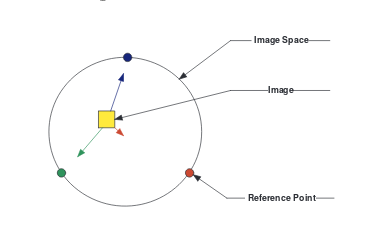
\includegraphics[scale=0.7]{imagenes/VCISR.png}  %el parámetro scale permite agrandar o achicar la imagen. En el nombre de archivo puede especificar directorios
\label{VCISR}
\caption{Puntos de atracción VCISR}
\end{figure}

Ahora veamos la representanción visual de una salida producida por una consulta.\\

\begin{figure}[H] %con el [H] le obligamos a situar aquí la figura
\centering
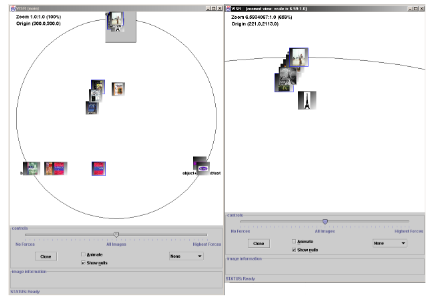
\includegraphics[scale=0.7]{imagenes/VCISR2.png}  %el parámetro scale permite agrandar o achicar la imagen. En el nombre de archivo puede especificar directorios
\label{VCISR}
\caption{Salida VCISR}
\end{figure}

Podemos apreciar como se distribuyen las imágenes a lo largo del círculo siguiendo el patrón comentado anteriormente.\\

Por otro lado podemos ver lo que ocurre al hacer zoom sobre una región. Al hacerlo apreciamos nuevas imágenes que permanecían ocultas.\\


\section{Fundamentos}

Este trabajo se basa en un sistema de recuperación de imágenes existente llamado \textit{Java Multimedia Retrival}, \textit{JMR}. Se trata de un \textit{CBIR} de código libre cuyo desarrollador principal e impulsor es el profesor Jesús Chamorro Martínez del departamento de Ciencias de la Computación e Inteligencia Artificial de la Universidad de Granada.\\

Se va hablar durante esta memoria sobre el espacio de color, por lo que es necesario darle una definición para saber a que nos referimos concretamente.\\

Por espacio de color nos referimos a un sistema de interpretación de color, una manera específica estructurar los colores de una imagen o vídeo. También es necesario hablar sobre los modelos de color, que se tratan de modelos matemáticos abstractos que describen la forma en la que cual los colores pueden ser representados como tuplas de números, normalmente como tres o cuatro valores o componentes de color, un ejemplo de esto sería RGB, en el que un color se descompone en tres valores, el valor de rojo, verde y azul.\\


\begin{figure}[H] %con el [H] le obligamos a situar aquí la figura
\centering
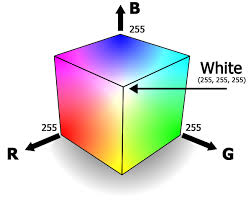
\includegraphics[scale=0.7]{imagenes/rgb.jpeg}  %el parámetro scale permite agrandar o achicar la imagen. En el nombre de archivo puede especificar directorios
\label{rgb.jpeg}
\caption{Modelo de color RGB}
\end{figure}

Otro ejemplo de espacio de color sería el \textit{HMMD}. Este espacio de color (Hue-Max-Min-Diff), es cercano a un espacio de color perceptualmente uniforme. Los nombres componentes, correspondientes a los distintos nombres, se pueden calcular a partir de RGB siguiente las siguientes transformaciones:

\begin{itemize}
\item \textbf{Max}: máximo(R,G,B)
\item \textbf{Min}: mínimo(R,G,B)
\item \textbf{Diff}: Max-min
\end{itemize}

Por otro lado, incluso se puede definir otro componente, llamado \texbf{Sum} = (Max+Min)/2.\\

En total habría una cantidad de 5 componentes en este espacio de color. Sin embargo, un cojunto de 3 elementos, {H,Max,Min} o {H,Diff,Sum}, es suficiente para para formar este espacio de color y especificar un punto de color.\\

\textit{Hue}, tiene la misma propiedad que su equivalente en el espacio de color HSV. \text{Hue} se mueve en el rango [0º, 360º]. \textit{Max} se mueve en el rango [0,1] y especifica cuanto color negro se encuentra presente, dando la sensación de sombra u oscuridad. \textit{Min}, rango [0,1], especifica cuanto color blanco se encuentra presente, dando la sensación de blanqueado. \textit{Diff}, rango [0,1], especifica como de cercano es un color a los colores puros, dando la sensación de tono o colorido. Finalmente, \textit{Sum}, especifica el brillo del color.
 
\begin{figure}[H] %con el [H] le obligamos a situar aquí la figura
\centering
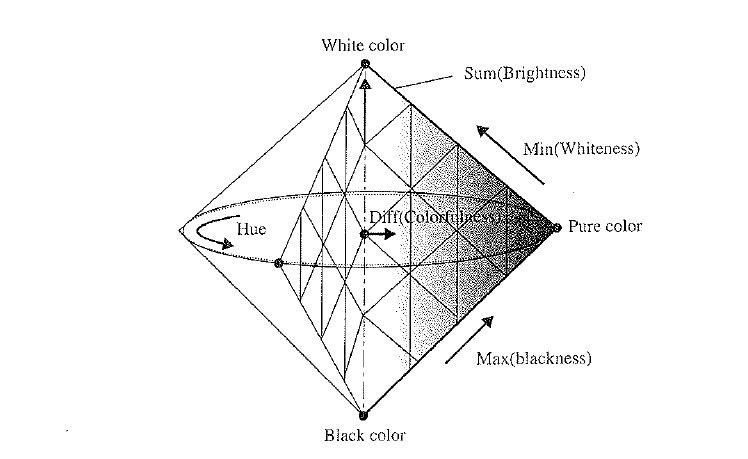
\includegraphics[scale=0.7]{imagenes/hmmd1.jpg}  %el parámetro scale permite agrandar o achicar la imagen. En el nombre de archivo puede especificar directorios
\label{hmmd1.jpg}
\caption{Modelo de color HMMD}
\end{figure}

\begin{figure}[H] %con el [H] le obligamos a situar aquí la figura
\centering
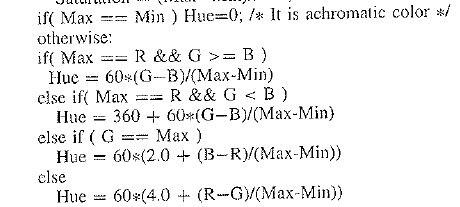
\includegraphics[scale=0.7]{imagenes/hmmd2.jpg}  %el parámetro scale permite agrandar o achicar la imagen. En el nombre de archivo puede especificar directorios
\label{hmmd2.jpg}
\caption{Cálculo Hue HMMD}
\end{figure}


Para este proyecto van a ser implementados una serie de descriptores. Estos descriptores se corresponden al tipo información general, previamente comentado, concretamente sobre el color. Estos son:

\begin{itemize}

\item Single Color Descriptor

\item MPEG7ColorStructure

\end{itemize}

\subsection{Single Color Descriptor}

Este descriptor de color se basa en el color medio de la imagen. Para calcularlo recorre una imagen en el espacio de color RGB píxel a píxel, obteniendo sus valores R, G y B. Cuando termina de recorrer todos los píxeles, calcula el color medio.

\subsection{MPEG7ColorStructure}

MPEG7ColorStructure es un descriptor de color que captura el contenido del color (similar a un histograma del color) e información sobre la estructura de este contenido. Su principal funcionalidad es la comparación imagen-imagen y se usa en la recuperación de imágenes, donde puede consistir una imagen de un solo marco rectangular o de forma arbitraria, posiblemente desconectado, regiones. El método de extracción incrusta información de estructura de color en el descriptor teniendo en cuenta todos los colores en un elemento estructurado de 8x8 píxeles que se desliza sobre la imagen, en lugar de considerar cada píxel por separado. A diferencia del histograma de color, este descriptor puede distinguir entre dos imágenes en las que un determinado color está presente en cantidades idénticas pero donde la estructura de los grupos de píxeles que tienen ese color es diferente en las dos imágenes. Los valores de color son dados por el ColorSpace MMD que se cuantifica de forma no uniforme en \textit{bin}, recipientes, de tamaño 32, 64, 128 o 256. Cada valor de amplitud de \textit{bin} está representado por un código de 8 bits. Este descriptor proporciona funcionalidad adicional y rendimiento en la recuperación de imágenes, basado en la similitud similitud, prsentando una mejora en comparación con el histograma de color ordinario.

\section{Objetivos}

Como todo proyecto que se realiza, este ha de tener una serie de objetivos que justifiquen su elaboración. Por lo que en este apartado se van a discutir los objetivos de este, dividiéndose en objetivos principales y secundarios.\\

Los principales, son los objetivos que el proyecto debe cumplir completamente. Mientras que los secundarios son objetivos que el proyecto no debe cumplir íntegramente, pero que en caso de hacerlo, suponen un gran valor añadido al proyecto. Cabe destacar que en este caso, los objetivos secundarios han sido satisfechos en su totalidad.\\

\subsection{Objetivos principales}

\begin{itemize}
  \item Desarrollar un sistema de recuperación de imágenes para plataformas móviles, para la plataforma Android concretamente. Actualmente el número de CBIR no es muy grande y no son muy conocidos por los usuarios, por lo que puede verse como una gran oportunidad.
  
  \item Este sistema debe ser capaz de permitir al usuario elegir la imagen consulta de su galería, o mediante la cámara del dispositivo, permitiendo realizar la consulta con dichas imágenes.
  
  \item Los resultados deben ser obtenidos en un periodo de tiempo aceptable. Esto ha de ser así, ya que en caso contrario, la experiencia del usuario se resentiría, lo que podría traducirse en un abandono de la aplicación.  
\end{itemize}


\subsection{Objetivos secundarios}

Una vez desarrollados los principales objetivos del proyecto, se explicarán los secundarios:

\begin{itemize}
  \item Utilizar una base de datos para almacenar los resultados. De esta manera, una vez calculada la primera consulta, el tiempo del resto se reduce drásticamente, lo que se traduce en una mejor experiencia para el usuario.

  \item Permitir al usuario modificar ajustes de la consulta. Logrando esto, el usuario puede adecuar la consulta a sus necesidades concretas, mejorando su experiencia con la aplicación.
\end{itemize}

%
\chapter{Objetivos}
\label{cap:objetivos}

Como todo proyecto que se realiza, este ha de tener una serie de objetivos que justifiquen su realización. Por lo que en este apartado se van a discutir los objetivos de este, diviendose en objetivos principales y secundarios.\\

Los principales son los objetivos que el proyecto debe cumplir completamente, mientras que los secundarios son objetivos que el proyecto no debe cumplir integramente, pero que en caso de cumplirlos, suponen un gran valor añadido al proyecto. Cabe destacar que en este caso, los objetivos secundarios han sido satisfechos en su totalidad.\\

\section{Objetivos principales}

\begin{itemize}
  \item Desarrollar un sistema de recuperación de imágenes para plataformas móviles, para la plataforma Android concretamente. Actualmente el número de CBIR no es muy grande y no son muy conocidos por los usuarios, por lo que puede verse como una gran oportunidad.
  
  \item Este sistema debe ser capaz de permitir al usuario elegir la imagen consulta de su galería, o mediante la cámara del dispositivo, permitiendo realizar la consulta con dichas imágenes.
  
  \item Los resultados deben ser obtenidos en un periodo de tiempo aceptable. Esto ha de ser así, ya que en caso contrario, la experiencia del usuario se resintiría, lo que podría traducirse en un abandono de la aplicación.  
  
\end{itemize}


\section{Objetivos secundarios}

Una vez desarrollados los principales objetivos del proyecto, se explicarán los secundarios:

\begin{itemize}
  \item Utilizar una base de datos para almacenar los resultados. De esta manera, una vez calculada la primera consulta, el tiempo del resto se reduce drásticamente, lo que se traduce en una mejor experiencia para el usuario.

  \item Permitir al usuario modificar ajustes de la consulta. Logrando esto, el usuario puede adecuar la consulta a sus necesidades concretas, mejorando su experiencia con la aplicación.
\end{itemize}

%
\chapter{Planificación}

\label{cap:planificacion}


Después de aclarar los objetivos del proyecto y requisitos del mismo, es tiempo de realizar la planificación.\\

Para realizar la planificación del proyecto disponemos de múltiples alternativas, pero en este caso la técnica a usar son los diagramas de Gantt. Un diagrama de Grantt puede ser considerado una herramienta visual en la cual se ve reflejado el tiempo que va a ser empleado en cada una de las tareas del proyecto.\\

La planificación de este proyecto ha sido dividida en varios bloques que serán comentados a continuación:

\section{Primer acercamiento}

Este bloque ha sido dedicado a un estudio preliminar sobre nociones básicas de \textit{Android}, para garantizar que las bases del proyecto fuesen correctas y así asegurarse de partir de una buena base. Por otro lado, una vez terminado dicho estudio, se empleó el resto del tiempo en asegurar la posibilidad de elegir la imagen consulta usando la galería, o mediante la cámara del dispositivo, cosa que puede complicarse si no se realiza correctamente.

Como detalle, mencionar que mi experiencia con \textit{Android} era poca, por lo que este primer acercamiento ha sido de gran importancia, ya que ha sentado las bases del proyecto.

\begin{figure}[H] %con el [H] le obligamos a situar aquí la figura
\centering
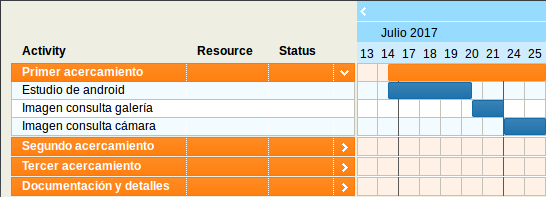
\includegraphics[scale=0.5]{imagenes/gant1.png}  %el parámetro scale permite agrandar o achicar la imagen. En el nombre de archivo puede especificar directorios
\label{gant1.png}
\caption{Diagrama Gantt. Primer acercamiento}
\end{figure}

El proyecto fue comenzado el 15 de julio. Los primeros días fueron empleados en el estudio de \textit{Android}, punto fundamental para empezar el proyecto. El resto de días se usaron para posibilitar la elección de la imagen consulta a través de la cámara o galería, gestionando los permisos de una forma adecuada.

\section{Segundo acercamiento}

Una vez establecido el punto de partida e instalado todo lo necesario pasamos al segundo bloque.\\

En este bloque se realizó un análisis para establecer cuales eran los requisitos necesarios para el correcto funcionamiento del proyecto.
Por otro lado, se desarrolló una interfaz prototipo, en la cual era posible seleccionar la imagen consulta, como hemos comentado anteriormente. Las imágenes consulta se mostraban en la parte superior de la pantalla, mientras que las imágenes resultado se mostraban en la parte inferior.\\

También se desarrolló un descriptor prototipo, para comprobar que realmente podíamos trabajar bien con las imágenes en \textit{Android}. Dicho descriptor únicamente cogía los píxeles de las imágenes y hacía cálculos triviales. Con esto, se estableció la estructura que debían tener los descriptores que se implementaron en el siguiente bloque.

\begin{figure}[H] %con el [H] le obligamos a situar aquí la figura
\centering
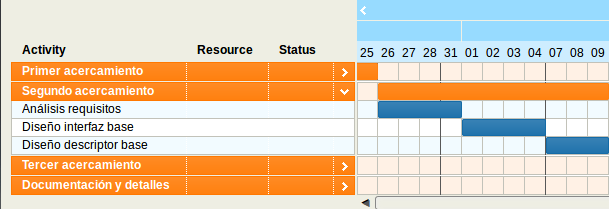
\includegraphics[scale=0.5]{imagenes/gant2.png}  %el parámetro scale permite agrandar o achicar la imagen. En el nombre de archivo puede especificar directorios
\label{gant2.png}
\caption{Diagrama Gantt. Segundo acercamiento}
\end{figure}

En este bloque el tiempo ha sido repartido de manera casi equitativa entre el análisis de requisitos, el diseño de la interfaz prototipo y del descriptor prototipo. Cosa crucial para la correcta realización del proyecto, ya que, aparte de implementar los prototipos, todos los requisitos deben estar establecidos antes de avanzar en el proyecto.\\

\section{Tercer acercamiento}

Este es el bloque al cual se le ha dedicado más tiempo en este proyecto, debido a que es en el que se ha procedido a la implementación de la interfaz final, de los descriptores y de la base de datos.\\

La interfaz sigue un estilo similar a la prototipo, con las imágenes consulta en la parte superior y en la inferior las imágenes resultado de la consulta. A su vez cuenta con otros apartados como ajustes e información adicional. Todo esto se comentará con detalle en su correspondiente sección.\\

Por el momento se han implementando dos descriptores:
\begin{itemize}
\item Media de color
\item Color estructurado
\end{itemize}

El primero se basa en el color medio de las imágenes, mientras que el segundo utiliza el histograma. Como en el caso de la interfaz, esto se detallará con más detalle.\\

Finalmente, después de todo lo anterior se decidió a implementar una pequeña base de datos que almacenase los valores obtenidos durante las consultas, de esta manera, en lugar de calcular el color medio o el histograma, se consultará en la base de datos y se obtendrá su valor, lo que reduce el tiempo de consulta drásticamente.\\

\begin{figure}[H] %con el [H] le obligamos a situar aquí la figura
\centering
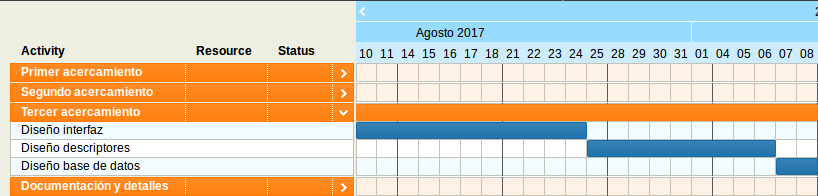
\includegraphics[scale=0.5]{imagenes/gant3.png}  %el parámetro scale permite agrandar o achicar la imagen. En el nombre de archivo puede especificar directorios
\label{gant3.png}
\caption{Diagrama Gantt. Tercer acercamiento}
\end{figure}


\section{Documentación y detalles}

En este último bloque se ha prodecido a la realización de esta memoria y a su vez a la revisión de todo el proyecto en busca de erratas y malfuncionamiento.\\

\begin{figure}[H] %con el [H] le obligamos a situar aquí la figura
\centering
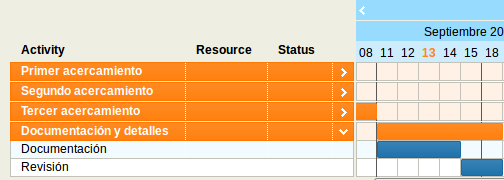
\includegraphics[scale=0.5]{imagenes/gant4.png}  %el parámetro scale permite agrandar o achicar la imagen. En el nombre de archivo puede especificar directorios
\label{gant4.png}
\caption{Diagrama Gantt. Documentación y detalles}
\end{figure}

Tras terminar todo el proyecto es muy importante revisarlo minuciosamente con el objetivo de encontrar fallos o elementos que se encuentren mal explicados. Por eso este bloque es gran importancia a pesar de ser el último.

%
\chapter{Metodología}
\label{cap:metodologia}

En este apartado se va a describir la metodología utilizada durante la realización de este proyecto. A su vez, se va a incluir una descripción de las herramientas, tecnologías y técnicas usadas, asi como de una justificación de dichas elecciones.


\section{Metodología}

Al comienzo de este proyecto se tuvieron varias reuniones para establecer los objetivos y requisitos que debía de cumplir este proyecto, aunque no en demasiada profundidad, siendo esto una tarea que se llevo a cabo según lo establecido en el capítulo anterior.\\

Una vez finalizadas dichas reuniones, se establecieron una serie de fechas en las cuales se tuvieron otras reuniones para comprobar el estado del proyecto. Estas fechas coinciden con la planificiación. De esta manera, se intercambiaron opiniones sobre la situación del proyecto, comentando posibles mejoras y solucionando las dudas surgidas durante las distintas etapas del desarrollo.\\

\section{Herramientas usadas}

En esta sección vamos a comentar las herramientas que han sido usadas durante la realización del proyecto.

\subsection{Android Studio}

Aunque no es estrictamente necesario para desarrollar aplicaciones Android, es posible utilizar eclipse por ejemplo, he decidio usarlo ya que es muy sencillo de entender y facilita al progamador muchas tareas. Esto ha sido muy importante ya que, como he comentado antes, mi experiencia con Android era muy reducida.\\

Android Studio es el entorno de desarrollo integrado, \textit{IDE}, oficial para la plataforma Android. Por esta razón la documentación es abundante, lo que supone un gran punto a su favor.\\

\begin{figure}[H] %con el [H] le obligamos a situar aquí la figura
\centering
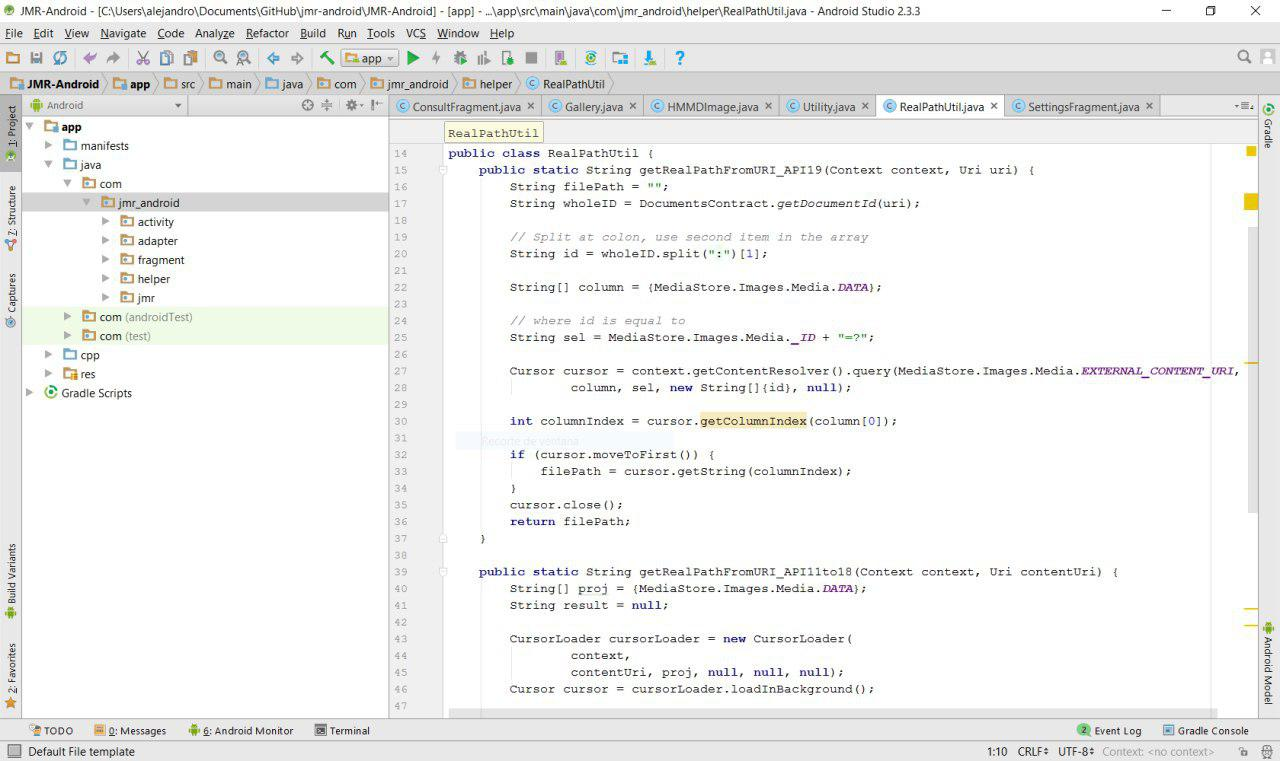
\includegraphics[scale=0.5]{imagenes/android-studio.jpg}  %el parámetro scale permite agrandar o achicar la imagen. En el nombre de archivo puede especificar directorios
\label{android-studio.jpg}
\caption{Ejemplo de proyecto Android Studio}
\end{figure}

Otra de las cosas interesantes de este \textit{IDE} es la posibilidad de diseñar interfaces de una manera muy sencilla e intuitiva, permitiendo arrastar los elementos a las posiciones deseadas. Por lo que no se requiere un gran nivel de programación para estas tareas. Aunque si hay que comentar, que si se necesita hacer cosas más complicadas, o que no sean las estándar, si es necesario un nivel de programación avanzado, ya que en dicho caso, la ayuda proporcionada por Android Studio para estas tareas se reduce.\\ 

\subsection{Git y GitHub}

Al tratarse de un proyecto de esta magnitud, ha sido necesario utilizar una herramienta de control de versiones, como es natural se ha utilizado git.\\

También se ha usado GitHub, que se trata de un lugar donde alojar nuestros proyectos utilizando el sistema de control de versiones Git. Por lo tanto, podemos entender que git y GitHub van de la mano, al menos en este caso.\\

El respositorio del proyecto se puede consultar \href{https://github.com/acasadoquijada/jmr-android}{aquí}.

Para llevar un control del proyecto se han usado los elementos conocidos como \textit{Milestones} y \textit{Issues} por GitHub.\\

Podemos entender un \textit{Issue} como una tarea por realizar, siendo un ejemplo, \textit{seleccionar imagen de la galería}. Se les puede añadir información extra, como a que \textit{Milestone} está asociado, que persona es la encargada de solucionarlo, o se puede añadir una etiqueta para establecer el tipo.\\

\begin{figure}[H] %con el [H] le obligamos a situar aquí la figura
\centering
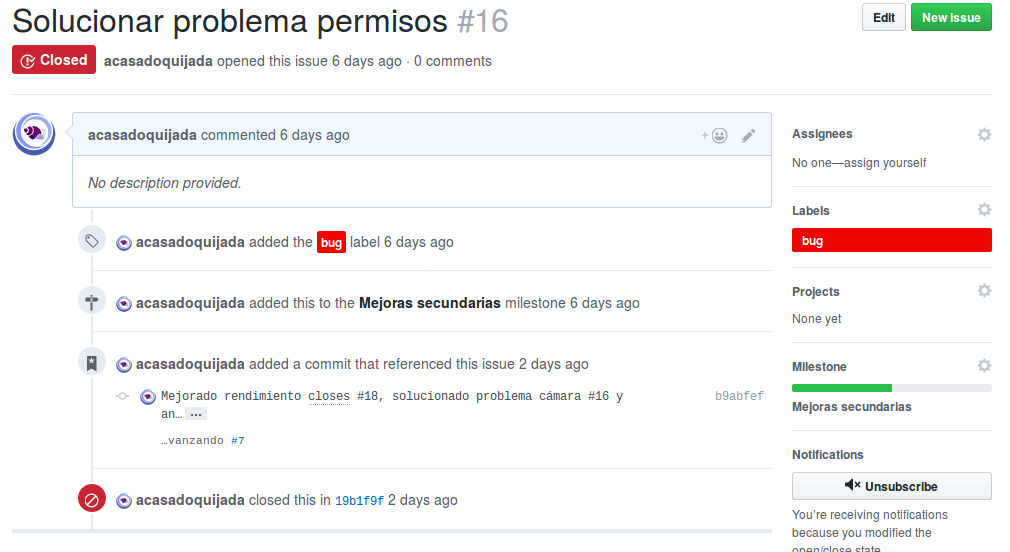
\includegraphics[scale=0.4]{imagenes/issue.png}  %el parámetro scale permite agrandar o achicar la imagen. En el nombre de archivo puede especificar directorios
\label{issue.png}
\caption{Ejemplo de issue}
\end{figure}

Por otro lado, se encuentran los \textit{Milestones}, que podemos considerarlos como hitos, es decir, un \textit{Milestone} está compuesto por varios \textit{Issues}. Por lo que también puede ser vistos como una agrupación de \textit{Issues}, una gran tarea dividida en pequeñas subtareas.\\

\begin{figure}[H] %con el [H] le obligamos a situar aquí la figura
\centering
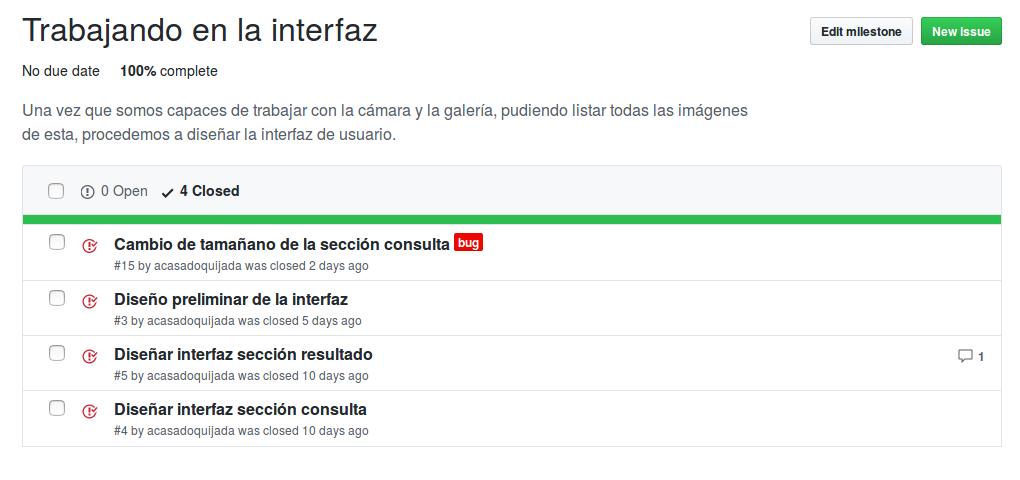
\includegraphics[scale=0.4]{imagenes/milestone.png}  %el parámetro scale permite agrandar o achicar la imagen. En el nombre de archivo puede especificar directorios
\label{milestone.png}
\caption{Ejemplo de milestone}
\end{figure}

Como se puede entender, usar ambos es de vital importancia si se desea llevar a cabo un proyecto de gran magnitud.
hablar sobre mi movil, carácterisiticas y tal

\subsection{Dispotivio de pruebas}

Aunque Android Studio nos ofrece la posibilidad de utilizar un emulador para lanzar la apliación, he decidido utilizar mi dispositivo movil, por motivos de eficiencia y comodidad. Debido a que no podía comprobar de manera real algunos aspectos de la propia aplicación, como el consumo de memoria o el propio rendimiento de las consultas.\\

Mi smartphone es un \textit{Xiaomi redmi 4 pro}, y cuenta con las siguientes características destacables:

\begin{itemize}
\item CPU: Qualcomm Snapdragon 625, con ocho núcleos y 2GHz 
\item Memoria: 3 GB
\item Almacenamiento: 32 GB
\end{itemize}

Se tratan de unas características que suelen ser habituales de encontrar en los smartphones actuales, por lo que ha sido un gran sujeto de pruebas.

\section{Tecnicas}

Para programar en Android se utiliza \textit{Java} para la lógica, y \textit{XML} para las interfaces de usuario.\\

Como es habitual, el desarrollo en Java ha seguido un paradigma de programación orientada a objetos, \textit{POO}. En el que se han desarrollado una serie de clases que se han organizado en distintos paquetes. Esto será explicado posteriormente.\\ 

Comentar que se ha utilizado también \textit{Android NDK}. Se trata de un conjunto de herramientas que nos permiten implementar partes de la aplicación en código nativo, como \textit{C} o \textit{C++}. Esta opción es perfecta para usar en los cálculos que realiza la aplicación. Como en el caso anterior se comentará con más detalle en su correspondiente sección.\\

\begin{figure}[H] %con el [H] le obligamos a situar aquí la figura
\centering
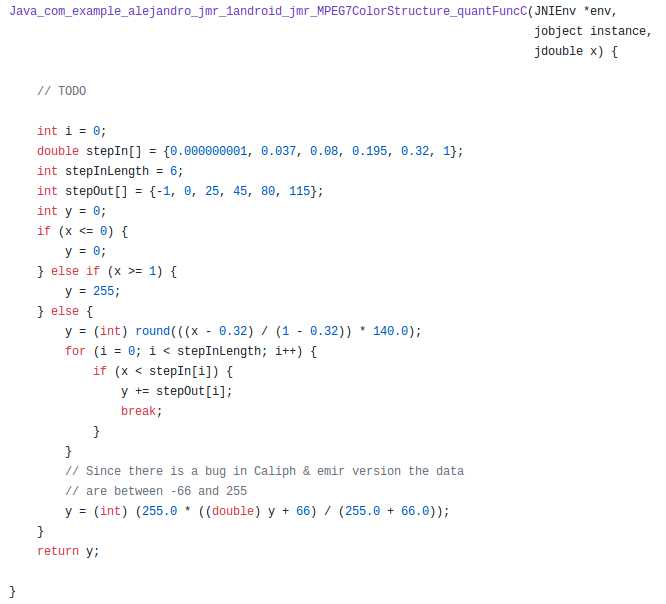
\includegraphics[scale=0.6]{imagenes/ndk.png}  %el parámetro scale permite agrandar o achicar la imagen. En el nombre de archivo puede especificar directorios
\label{ndk.png}
\caption{Ejemplo de código Android ndk}
\end{figure}

Por último comentar que se ha usado \textit{XML} para las interfaces de usuario, la mayor parte del tiempo apoyándose en el soporte proporcionado por Android Studio, pero que a la hora de realizar cosas mas complejas se ha tenido que escribir manualmente dicho código XML.

\begin{figure}[H] %con el [H] le obligamos a situar aquí la figura
\centering
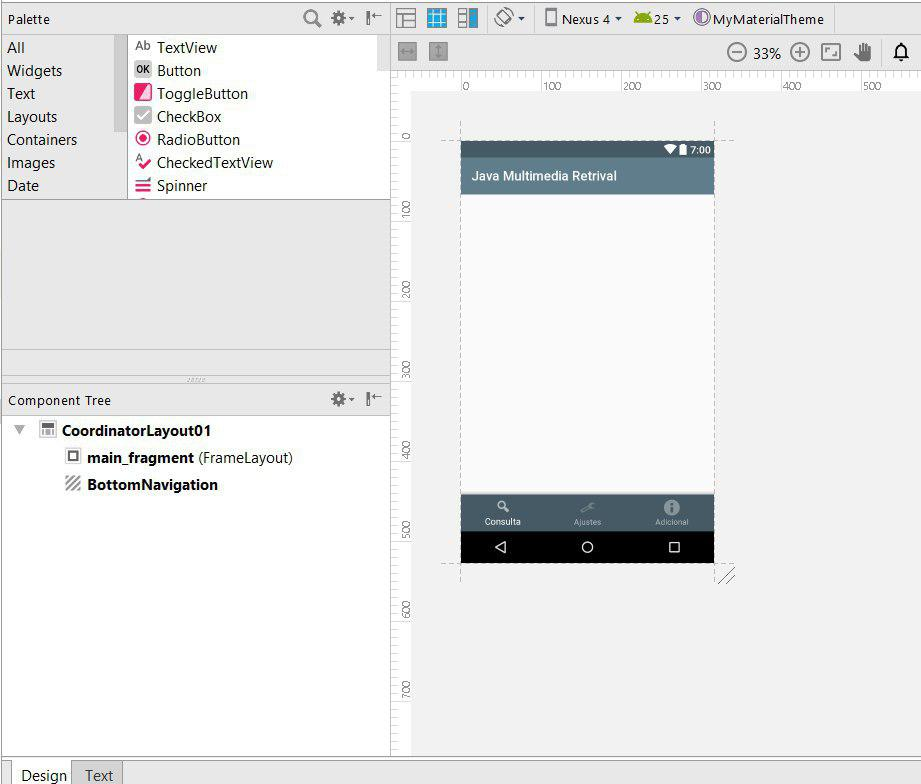
\includegraphics[scale=0.6]{imagenes/interfaz-android-studio.jpg}  %el parámetro scale permite agrandar o achicar la imagen. En el nombre de archivo puede especificar directorios
\label{interfaz-android-studio.jpg}
\caption{Ejemplo de proyecto Android Studio}
\end{figure}

%
\chapter{Desarrollo}
\label{cap:desarrollo}

En este capítulo se va a llevar a cabo el estudio del arte relativo a este proyecto y se van a comentar el proceso realizado para conseguir los objetivos establecidos.

\section{Estudio del arte}

El estudio del arte debe hacerse por partida doble. Debe estudiarse el estado en el que se encuentra Android y a parte, los \texit{CBIR} en dicha plataforma.\\

\subsection{Estado arte Android}

Por la parte de la lógica no hay ningún tipo de misterio, ya que tratamos con Java y XML, cosas que apenas cambian y ya se tienen muy estudiadas e asimiladas, por lo que no es necesario un gran estudio de esta parte.\\

Lo que si hay que tener en cuenta es el desarrollo de interfaces de usuario. Este es un tema muy importante, ya que aunque la aplicación funcione correctamente y presente unas novedades increibles, un mal diseño de interfaz puede provocar su abando por parte de los usuarios. Resulta natural dedicar un tiempo de investigación a esta parte.\\

\subsubsection{Material design}
Al realizar cualquier búsqueda sobre diseño de interfaces en Android nos encontramos con \textit{Material design}, que se trata de una guía integral para el diseño visual, de movimientos y de interacción en distintas plataformas y dispositivos. Presenta una gran serie de nuevos elementos y novedades. Actualmente es el estándar de Android. Debido a esto, se debe seguir \textit{Material design} a la hora de realizar una interfaz.

\begin{figure}[H] %con el [H] le obligamos a situar aquí la figura
\centering
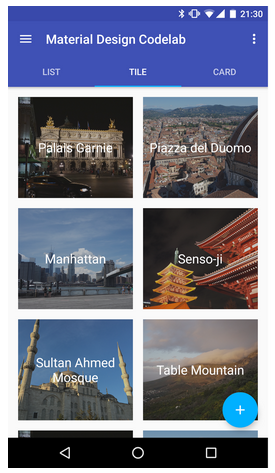
\includegraphics[scale=0.5]{imagenes/desing1.png}  %el parámetro scale permite agrandar o achicar la imagen. En el nombre de archivo puede especificar directorios
\label{design1}
\caption{Ejemplo de Material Design 1}
\end{figure}

\begin{figure}[H] %con el [H] le obligamos a situar aquí la figura
\centering
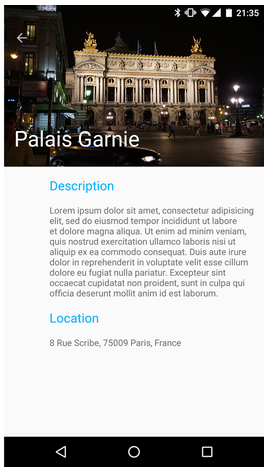
\includegraphics[scale=0.5]{imagenes/desing2.png}  %el parámetro scale permite agrandar o achicar la imagen. En el nombre de archivo puede especificar directorios
\label{design1}
\caption{Ejemplo de Material Design 2}
\end{figure}

Tras un estudio preliminar de \textit{Material design} se procedió a estudiar con más detalle dos elementos. Estos son \textit{floating action button}, \textit{Bottom Navigation} y \textit{Glide}.

\subsubsection{Floating action button}

Un \textit{Floating action button} representa la acción principal en una aplicación. Normalmente se encuentra en forma de un icono en cicular que se encuentra flotando sobre la interfaz de usuario, cambia de color al pulsar y se eleva al seleccionar. Cuando se presiona, puede contener más acciones relacionadas.\\

En mi caso he utilizado la implementación usada por \textit{Clans}, el código fuente se puede encontrar en su \href{https://github.com/Clans/FloatingActionButton}{repositorio}

\begin{figure}[H] %con el [H] le obligamos a situar aquí la figura
\centering
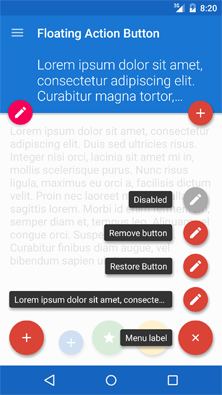
\includegraphics[scale=0.5]{imagenes/fab.png}  %el parámetro scale permite agrandar o achicar la imagen. En el nombre de archivo puede especificar directorios
\label{fab}
\caption{Ejemplo Floating action button}
\end{figure}

\subsubsection{Bottom Navigation}

Los \textit{Bottom Navigation} nos proporciona una navegación rápida entre las vistas de nivel superior de una aplicación. Está diseñado principalmente para su uso en dispositivos móviles. Las pantallas más grandes, como el escritorio, pueden lograr un efecto similar usando la navegación lateral. Por ejemplo, el tratamiento compacto "rail" muestra los iconos de navegación de forma predeterminada.\\

En mi caso he utilizado la implementación usada por \textit{sephiroth74}, el código fuente se puede encontrar en su \href{https://github.com/sephiroth74/Material-BottomNavigation}{repositorio}\\

\begin{figure}[H] %con el [H] le obligamos a situar aquí la figura
\centering
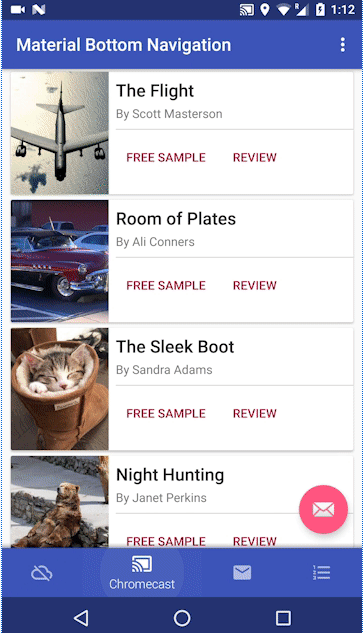
\includegraphics[scale=0.5]{imagenes/mbottom.png}  %el parámetro scale permite agrandar o achicar la imagen. En el nombre de archivo puede especificar directorios
\label{mbottom}
\caption{Ejemplo Bottom Navigation}
\end{figure}

\subsubsection{Glide}

Se trata de un marco de trabajo rápido y eficiente de código abierto que se encarga de la gestión de imágenes, agrupando la decodificación de medios, la gestión de memoria y el almacenamiento de cache en disco mediante una interfaz simple y sencilla de utilizar.\\

Actualmente se encuentra recomendada por \textit{Google}, está desarrollada por \textit{Bump Technologies}, y se puede consultar en el enlace de su \href{https://github.com/bumptech/glide}{repositorio}\\


\begin{figure}[H] %con el [H] le obligamos a situar aquí la figura
\centering
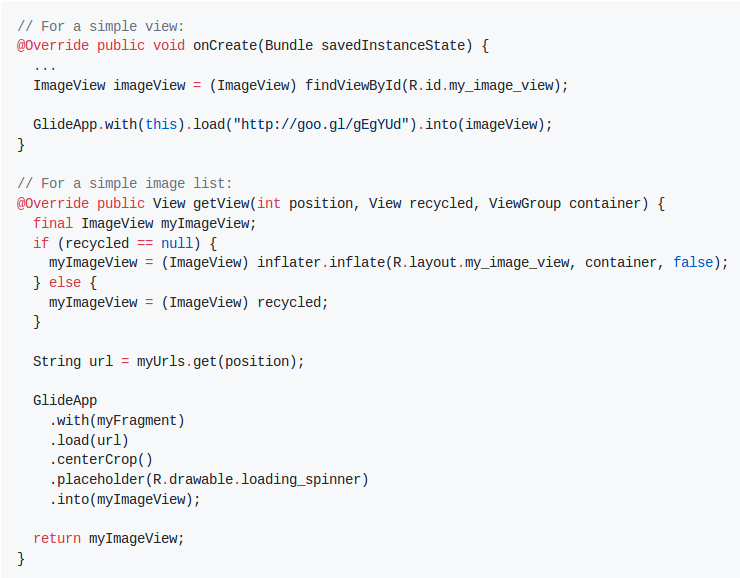
\includegraphics[scale=0.5]{imagenes/glide.png}  %el parámetro scale permite agrandar o achicar la imagen. En el nombre de archivo puede especificar directorios
\label{glide}
\caption{Ejemplo de uso de Glide}
\end{figure}

En nuestro caso es ideal, ya que nos proporciona una manera sencilla de trabajar con imágenes y a su vez, nos permite utilizar movimientos de desplazamiento scroll de una manera simple, lo que nos posibilita centrarnos en la manera en la que queremos representar las imágenes.

\subsection{Estado CBIR Android}

Lo primero que podemos encontrar es información abundante sobre CBIR en computadores, pero en nuestro caso no nos es necesaria, ya que partimos de uno previo, Java Multimedia Retrival, que cuenta con todo lo que necesitamos sobre este tipo de sistemas. Aunque siempre es interesante estar al día en estos asuntos.\\

Por lo que vamos a centrarnos en los CBIR desarrollados exclusivamente para sistemas Android, sin embargo, si vamos a comentar el CBIR Java Multimeda Retrieval, ya que partimos de él.

\subsubsection{Java Multimedia Retrieval}

Se trata de un CBIR desarrollado en Java, iniciado por Jesus Chamorro, profesor de la universidad de Granada.\\

Este CBIR trabaja con 3 descriptores distintos, basados en el color dominante, estructurado y escalable. Nos ofrece la posibilidad de realizar las consultas con cualquiera de dichos descriptores, incluso con 2 o 3 a la vez. A su vez cuenta con una pequeña base de datos donde se almacenan los resultados de las consultas para agilizar las posteriores.

\begin{figure}[H] %con el [H] le obligamos a situar aquí la figura
\centering
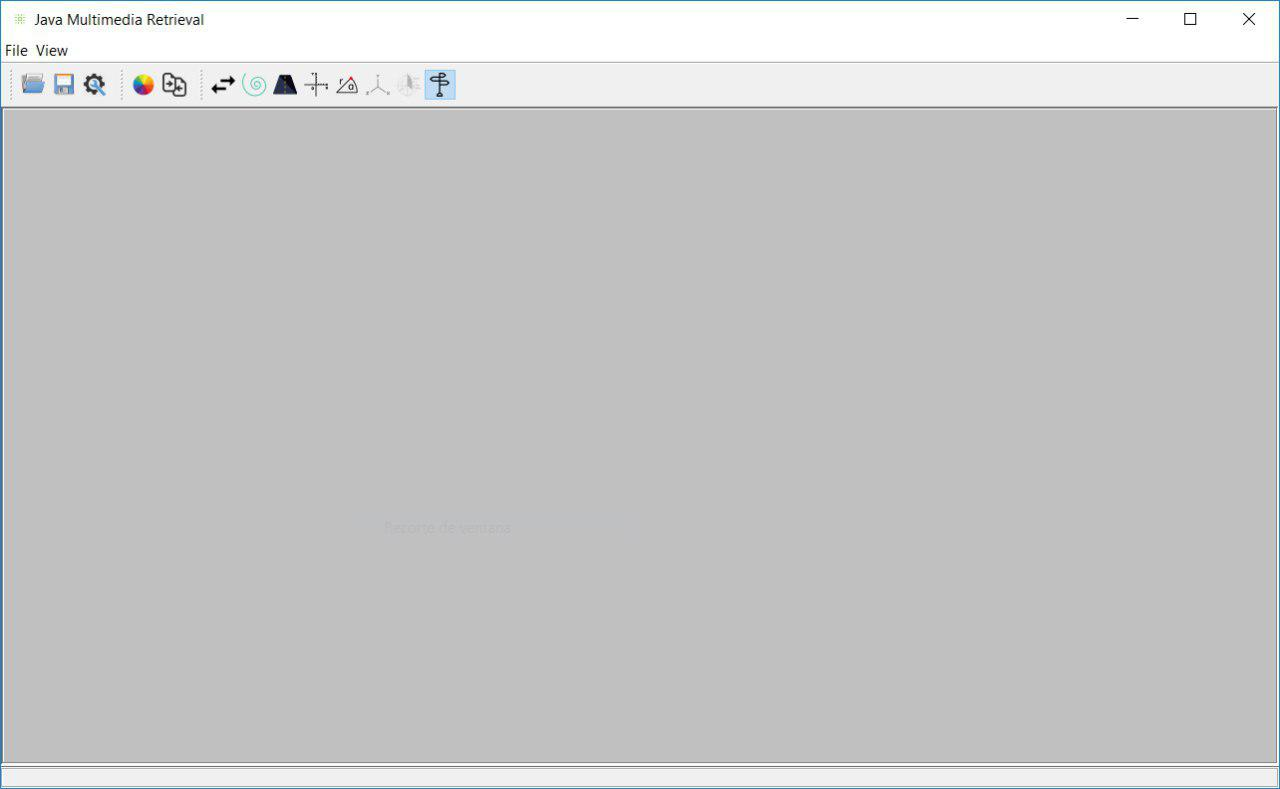
\includegraphics[scale=0.5]{imagenes/jmr.jpg}  %el parámetro scale permite agrandar o achicar la imagen. En el nombre de archivo puede especificar directorios
\label{jmr}
\caption{Interfaz Java Multimedia Retrieval}
\end{figure}

\subsubsection{Content based image retrieval for mobile systems}

En esta ocasión nos encontramos ante un artículo escrito por \textit{P Jeyanthi} profesor asociado del departamento de tecnologías de la información de la universidad Sathyabama, Rajiv Gandhi Salai, India.\\

En el artículo se habla sobre un enfoque para la realización de la extracción de características basadas en textura por la co-ocurrencia de nivel de gris y la matriz de color basado en la extracción de características por color vector de concurrencia. La mayor parte del artículo se centra en el cálculo de descriptores, cosa que como se ha mencionado antes, a nosotros no nos es relevante. Por otro lado podemos ver un poco de la interfaz, lo que si nos interesa, aunque comprobamos de que se trata de una interfaz muy pobre, ya que se concentran en el cálculo de descriptores más que en la representación de los resultados.


\begin{figure}[H] %con el [H] le obligamos a situar aquí la figura
\centering
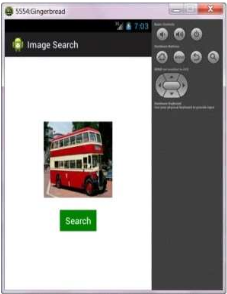
\includegraphics[scale=0.6]{imagenes/articulo11.png}  %el parámetro scale permite agrandar o achicar la imagen. En el nombre de archivo puede especificar directorios
\label{articulo11}
\caption{Interfaz CBIR for mobile systems 1}
\end{figure}

\begin{figure}[H] %con el [H] le obligamos a situar aquí la figura
\centering
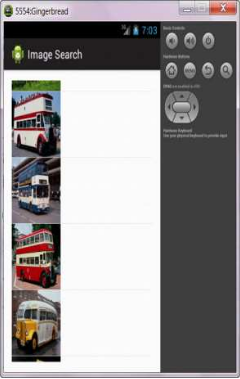
\includegraphics[scale=0.6]{imagenes/articulo12.png}  %el parámetro scale permite agrandar o achicar la imagen. En el nombre de archivo puede especificar directorios
\label{articulo11}
\caption{Interfaz CBIR for mobile systems 2}
\end{figure}

Otro de los aspectos que nos interesan es el tiempo de cómputo y el consumo de recursos, pero no se hace ningún tipo de referencia a estos aspectos en el artículo.\\

Tras realizar un estudio del estado del arte de los CBIR en Android podemos llegar a la conclusión de que se tratan de sistemas que han sido poco explotados en dicha plataforma, y lo más importante, el usuario medio no conoce de su existencia, por lo que este proyecto cubre un espacio de mercado que se encuentra desocupado.\\

\section{Proceso de desarrollo}

En esta sección vamos a detallar los distintos elementos que componen el proyecto con un nivel de detalle suficiente para dar una visión global del proyecto y entender cada uno de sus componentes.\\

Como visión global podemos ver la aplicación como una única actividad que va cambiando el fragment que se muestra en pantalla, cada fragment se encarga de sus propias tareas, dejando a la actividad encargándose únicamente de cambiar fragments y otras cosas triviales.

\subsection{Paquetes}

Vamos a comenzar hablando de los distintos paquetes de los que se compone el proyecto.

\begin{figure}[H] %con el [H] le obligamos a situar aquí la figura
\centering
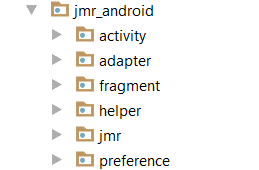
\includegraphics[scale=0.9]{imagenes/paquetes.jpg}  %el parámetro scale permite agrandar o achicar la imagen. En el nombre de archivo puede especificar directorios
\label{paquetes}
\caption{Paquetes del proyecto}
\end{figure}

\subsubsection{Activity}

En él se cuentran las activities que forman parte del proyecto. En este caso solo forma parte de él una única actividad, \textit{MainActivity} que es la encarga de gestionar la aplicación.

\subsubsection{Adapter}

Formado por \textit{GalleryAdapter} y \textit{ViewPagerAdapter}. El primero se encarga de renderizar las imágenes para su correcta visualización, mientras que el segundo se encarga se usa para permitir que podamos interactuar con las imágenes.

\subsubsection{Fragment}

En este paquete se encuentan los distintos framgents de los que se componen el proyecto, un total de 4. Los tres primeros se corresponden a cada una de las opciones del menú inferior de la aplicación, mientras que el último se encarga de que podamos interactuar con las imágenes al pulsar sobre ellas, aportandónos información.

\subsubsection{Helper}

Formado por clases que se encargan de \textit{ayudar} al resto para que su funcionamiento sea el esperado. Entre algunos de los miembros de este paquete destacan \textit{DBHelper}, que se encarga de la gestión de la base de datos y \textit{GalleryHelper}, encargado de la gestión de la galería del usuario.

\subsubsection{JMR}

Paquete en el que se encuentra todo lo relacionado con el cálculo de descriptores y la organización de sus resultados. A su vez cuenta con clases como \textit{HMMDImage} que se encarga de pasar una imagen en el espacio de color \textit{RGB} al espacio de color \textit{HMMD}. Esto se explicará con detalle en el próximo apartado

\subsection{Clases}

Una vez que se ha terminado de hablar de los paquetes, es hora de hablar de cada clase individualmente. Al igual que en el caso anterior, lo haremos con cierto nivel de detalle, sin entrar en cuestiones demasiado técnicas.

\subsubsection{MainActivity}

Es la única clase actividad, \textit{Activity}, del proyecto. Se encarga de instanciar e iniciar las 3 clases \textit{Fragment} que se corresponden a cada una de las opciones del menú inferior. A su vez, se ocupa de la comunicación entre \textit{Fragments}, necesaria para un correcto funcionamiento de la aplicación, y también se ocupa de gestionar la memoria, para evitar que la aplicación ocupe demasiados recursos. Esto se consigue controlando la cola de \textit{Fragments} de la aplicación.

\subsubsection{GalleryAdapter}

Esta clase se encarga de \textit{hinchar}, \textit{inflate}, un fichero XML llamado gallery_thumbnail.xml, en el cuál se colocan las imágenes, una por cada instancia del fichero, y a su vez, se encarga de reenderizar las imágenes. Se puede decir, que esta clase se encarga de colocar todas las imágenes y nos permite interactuar con ellas a través de eventos.

\subsubsection{ConsultFragment}

Clase de tipo \textit{Fragment} que puede considerarse como el núcleo del proyecto.\\

En ella se inicializa su propia interfaz, al igual que el resto de sus clases \textit{Fragment} hermanas. Garantiza que el usuario pueda elegir la imagen consulta tanto de la cámara como de la galería, estas imágenes se van acumulando en la parte superior de la pantalla, pudiendo moverse realizando un movimiento de scroll. También gestiona los permisos, ya que es aquí donde se encuentran los métodos que requieren de ellos para poder desempeñar correctamente su función.\\

Todos los cálculos de descriptores son realizados aquí, consultado previamente si los valores a calcular se encuentran en la base de datos y actuando en consecuencia. Para estos cálculos se utilizan las clases que se encuentran en el paquete JMR. Las imágenes resultantes de una consulta, imágenes resultado, se colocan justo debajo de las imágenes consulta, en cuatro columnas, pudiendo realizar un movimiento de scroll en caso de que no cupiesen todas en la pantalla del dipositivo.

\subsubsection{SettingsFragment}

Esta clase se encarga de gestionar el apartado de opciones de la aplicación. Permite al usuario elegir con que descriptor desea realizar las consultas, entre otras cosas. Básicamente, a través de eventos recoge las acciones del usuario y se las transmite a otras clases, en caso de ser necesario, usando la clase \textit{MainActivity}.\\

Un ejemplo de esto es cuando el usuario decide cambiar el descriptor activo. En esa ocasión, esta clase notifica a \textit{ConsultFragment} utilizando a \textit{MainActivity}

\subsubsection{SlideshowDialogFragment}

Esta clase, junto con su clase interna adapter, \textit{MyViewPageAdapter}, nos proporciona los métodos necesarios para que, cuando pulsemos una imagen, esta aparezca ocupando toda la pantalla y a su vez, nos muestra información sobre ella. Esta información es el número de imagen que ocupa del total, imagen 5 de 400, y la distancia de la imagen consulta, un valor entre 0 y 1 que nos indica como de parecidas son las imágenes entre si, siendo 0 iguales y 1 totalmente distintas.

\subsubsection{Fragment sobre nosotros}

Poner licencias, que hable un poco del proyecto.
 
\subsubsection{DBHelper}

Clase encargada de la gestión de la base de datos. Cuenta con métodos para crearla, alterarla y destruirla. Cuando se están realizando los cálculos de los descriptores, se consulta la base de datos a través de los métodos de esta clase, para comprobar si el valor que se desea calcular se encuentra en ella, o en caso contrario, introducirlo. Esta base de datos es de tipo relacional.

\subsubsection{GalleryHelper}

Se encarga de gestionar todas las imágenes disponibles en el dispositivo del usuario, como es natural pensar, requiere de permisos por parte de él. Dispone de todo tipo de métodos para obtener las imágenes, y para minimizar el consumo de recursos lo único que se mantiene en memoria es la ruta de las imágenes, \textit{path}. Cuando es necesario cargar una imagen, se hace en base a su ruta, lo que evita tener todas las imágenes en memoria, un escenario que sería imposible.

\subsubsection{RealPathUtil}

Clase que se ocupa de tratar la ruta o \textit{path} de las imágenes, tarea que puede resultar trivial, pero no lo es.

\subsubsection{SquareLayout}

En esta ocasión, esta clase extiende de \textit{RelativeLayout} y se encarga de representar una imagen de manera cuadrada en un \textit{grid view}, es decir, en las 4 columnas de las que hablabamos previamente.

\subsubsection{Utility}

Se encarga de gestionar los permisos que necesitan el resto de clases para actuar correctamente. Cuando una clase requiere cualquier tipo de permiso se pone en contacto con ella y actua en consecuencia.

\subsubsection{HMMDImage}

Dado que el descriptor \textit{MPEG7ColorStructure} necesita que la imagen en el espacio de color HMMD, esta clase se encarga de dicha tarea. Utiliza una imagen en espacio de color RGB y la transforma HMMD, con una serie de operaciones matemáticas no muy complejas.

\subsubsection{JMRImage}

Siempre que nos referimos a imagen, nos referimos a esta clase. Cuenta con todo lo necesario para garantizar que el consumo de memoria sea lo mínimo posible, como se ha comentado anteriormete. Simplemente guarda información sobre la imagen, pero no a la propia imagen. Esta información es utilizada a la hora de cargar la imagen, y de añadirle más nivel de detalle, tal que el número de la imagen respecto a las demás o su distancia a la imagen consulta, en caso de que se trate de una imagen resultado.

\subsection{MPEG7ColorStructure}

Clase que representa al descriptor de mismo nombre y que utiliza el histograma de una imagen en espacio de color HMMD, que posteriormente se comparará con el resto de histogramas del resto de las imágenes para ver cuan parecidas son entre ellas.

\subsection{ResultList}

Extiende de \textit{







Hablar de los disintos paquetes del proyecto. Aqui meter diagrama

Hablar de las clases, que hacen y sus principales métodos. Aqui meter diagrama

historias de usuario. 






%
\chapter{Resultados}
\label{cap:resultados}

\section{Tamaños y tiempos}
Lo primero que debemos considerar como resultado, es el tiempo de ejecución de la aplicación, ya que nos encontramos ante un dispositivo movil, que no dispone de la misma cantidad de recursos que un ordenador portatil o de sobremesa.\\

También hay que tener en cuenta que estamos trabajando con imágenes, por lo que a mayor cantidad de píxeles de esta, mayor será el tiempo de cómputo, por lo que se debe encontrar un equilibrio entre el tamaño de las imagénes y el resultado obtenido. De nada nos sirve que la aplicación tarde muy poco tiempo en comparar un gran número de imágenes si el resultado es totalmente erroneo.\\

En una serie de pruebas iniciales, el tamaño de las imágenes no se tuvo en cuenta, por lo que incluso con el descriptor prototipo, no realizaba níngún tipo de cálculo, los tiempos de consulta eran demasiado elevados, a pesar de usar un número pequeño de imágenes.\\

El siguiente paso fue redimensionar las imágenes a un tamaño concreto, se comenzó con 200x200. Con este tamaño se redujo el tiempo de cómputo, y los resultados comenzaban a ser prometedores. Pero se comprobó que el tiempo de cómputo crecía demasiado con el número de imágenes, por lo que se descartó este tamaño.\\

Con los tamaños 64x64 y 32x32, este último es el definitivo, se obtuvieron unos buenos tiempos de ejecución y unos buenos resultados, aunque se decidió usar 32x32 ya que el descriptor MPEG7, realiza una gran cantidad de operaciones con el histograma de la imagen, por lo que ese tamaño se adapta mejor a nuestras necesidades. Se probaron estos dos últimos tamaños, ya que en una asignatura de este máster se tuvo que trabajar con imágenes, y dichos tamaños, son los que mejores resultados nos proporcionaron.\\

\section{Consultas}

Una vez discutidos los tiempos y tamaños, es hora de comprobar que los resultados de las consultas son los esperados. Para ello vamos a utilizar dos bases de imágenes:\\

\begin{itemize}

\item Banderas. Un cojunto de 160 con las banderas de los principales países del mundo.

\item VisTex. Conjunto de imágenes de texturas, constituida por un total de 669 elementos.

\end{itemize}

\begin{figure}[H] %con el [H] le obligamos a situar aquí la figura
\centering
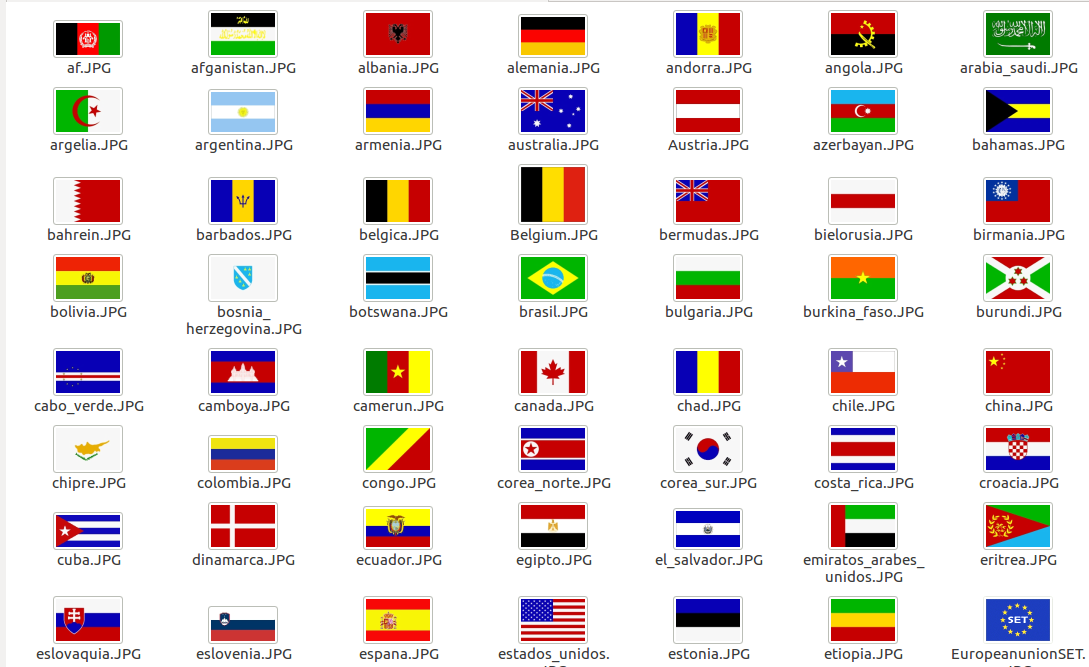
\includegraphics[scale=0.4]{imagenes/banderas.png}  %el parámetro scale permite agrandar o achicar la imagen. En el nombre de archivo puede especificar directorios
\label{banderas}
\caption{Base de datos de banderas}
\end{figure}

\begin{figure}[H] %con el [H] le obligamos a situar aquí la figura
\centering
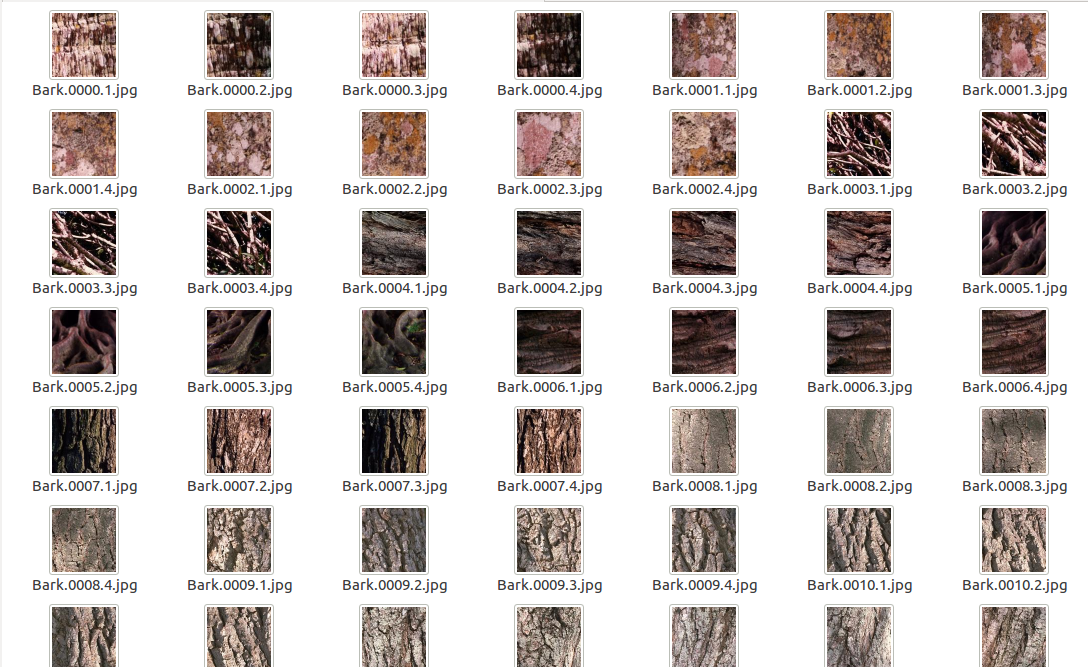
\includegraphics[scale=0.4]{imagenes/texturas.png}  %el parámetro scale permite agrandar o achicar la imagen. En el nombre de archivo puede especificar directorios
\label{texturas}
\caption{Base de datos de VisTex}
\end{figure}

Como es natural, también se han realizado las pruebas con imágenes propias de mi dispositivo, pero por comodidad y para ver mejor los resultados se ha decidido usar estas dos bibliotecas.


\subsection{Color medio}

Hablar sobre el color medio, y poner resultados usando las imágenes bandera, y vistex. 2/4 pantallazos


\subsection{MPEG7}

Hablar sobre el MPEG7, y poner resultados usando las imágenes banedra y vistex. 2/4 pantallazos






%
\input{capitulos/08_Conclusiones}
%
%%\chapter{Conclusiones y Trabajos Futuros}
%
%
\nocite{*}
\bibliography{bibliografia/bibliografia}\addcontentsline{toc}{chapter}{Bibliografía}
\lhead{\textsc{Bibliograf\'ia}} % Change the page header to say "Bibliografía"
\bibliographystyle{plain}
%
\appendix
%\chapter{Manual de usuario}
\label{cap:Manual de usuario}

\section{Permisos}

Para el correcto funcionamiento de la aplicación es necesario que el usuario de permisos a la aplicación para poder acceder tanto a la cámara, como a las imágenes del dispositivo.\\

Al iniciar la aplicación se nos pedirá permiso para acceder al contenido del teléfono, ya que es en ese instante, cuando se inicia la aplicación, el momento en el que se listan todas las imágenes del dispositivo.

\begin{figure}[H] %con el [H] le obligamos a situar aquí la figura
\centering
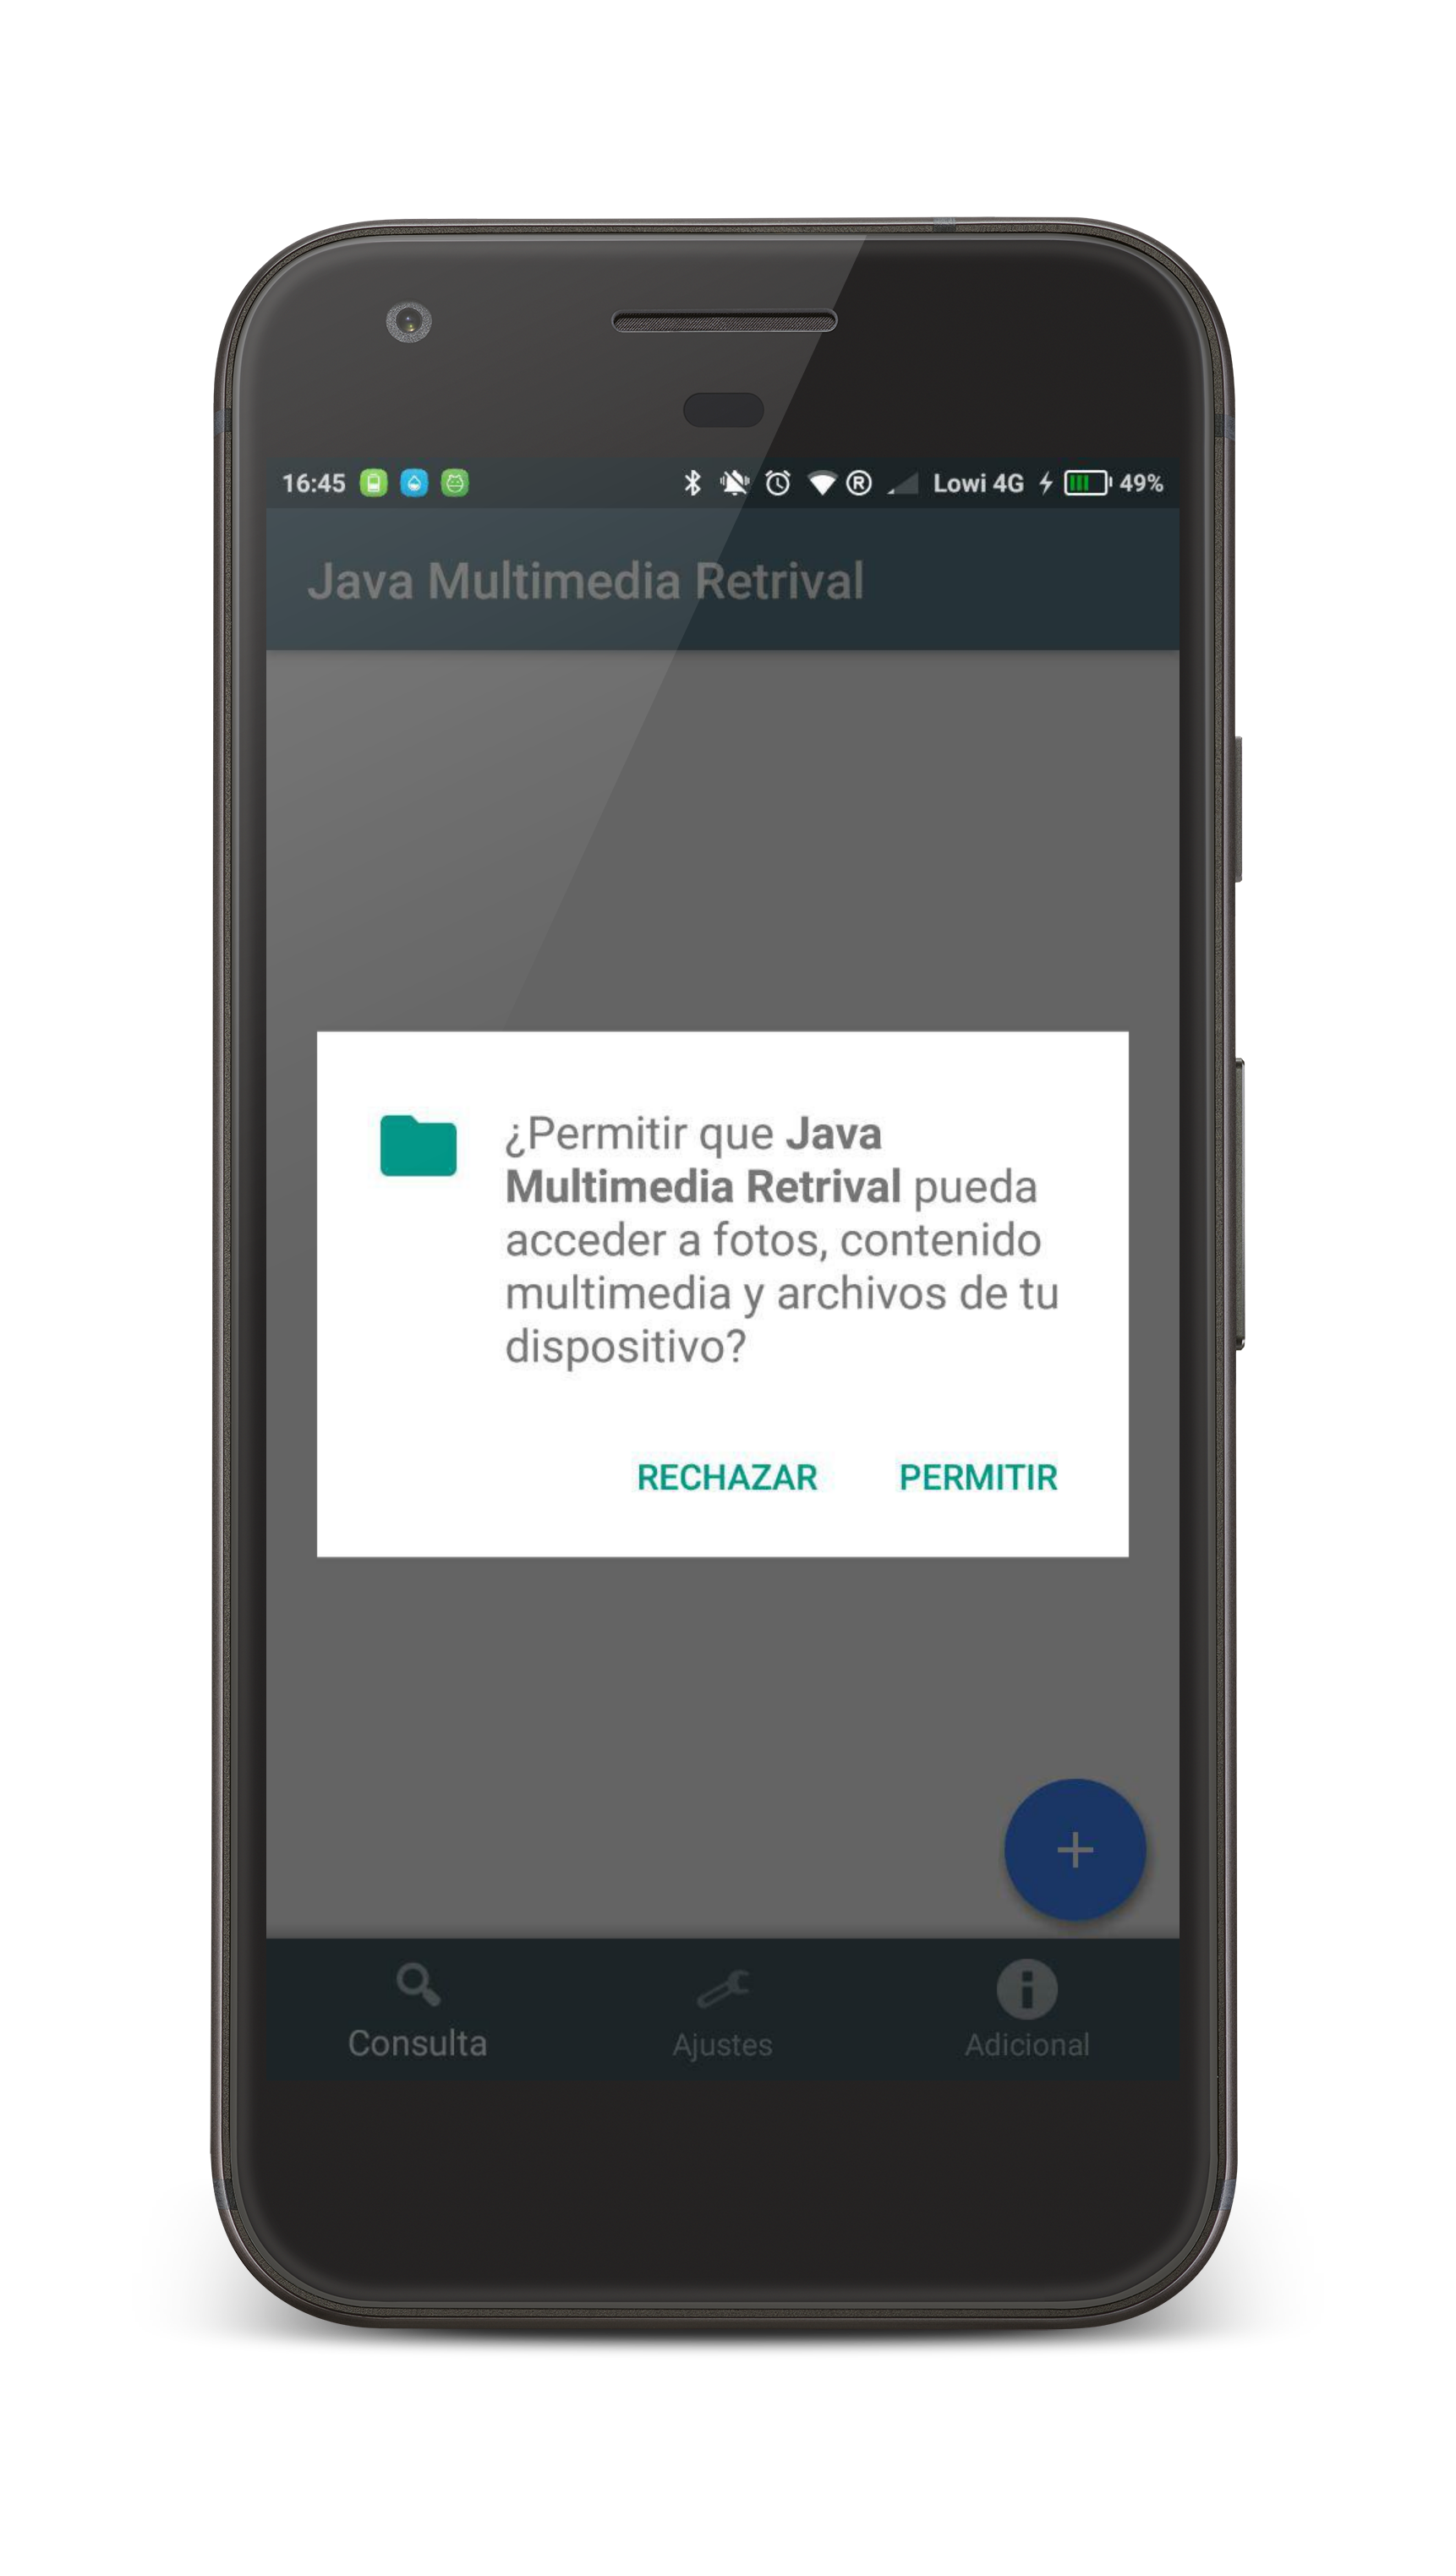
\includegraphics[scale=0.15]{imagenes/permisos1.png}  %el parámetro scale permite agrandar o achicar la imagen. En el nombre de archivo puede especificar directorios
\label{permisos1.png}
\caption{Permisos aplicación 1}
\end{figure}

En caso de no conceder el permiso, cuando intentemos acceder al recurso otra vez, galería o cámara, se nos volverá a preguntar. Una vez aceptado, ya podemos acceder a los recursos requeridos sin ningún tipo de problema.

\begin{figure}[H] %con el [H] le obligamos a situar aquí la figura
\centering
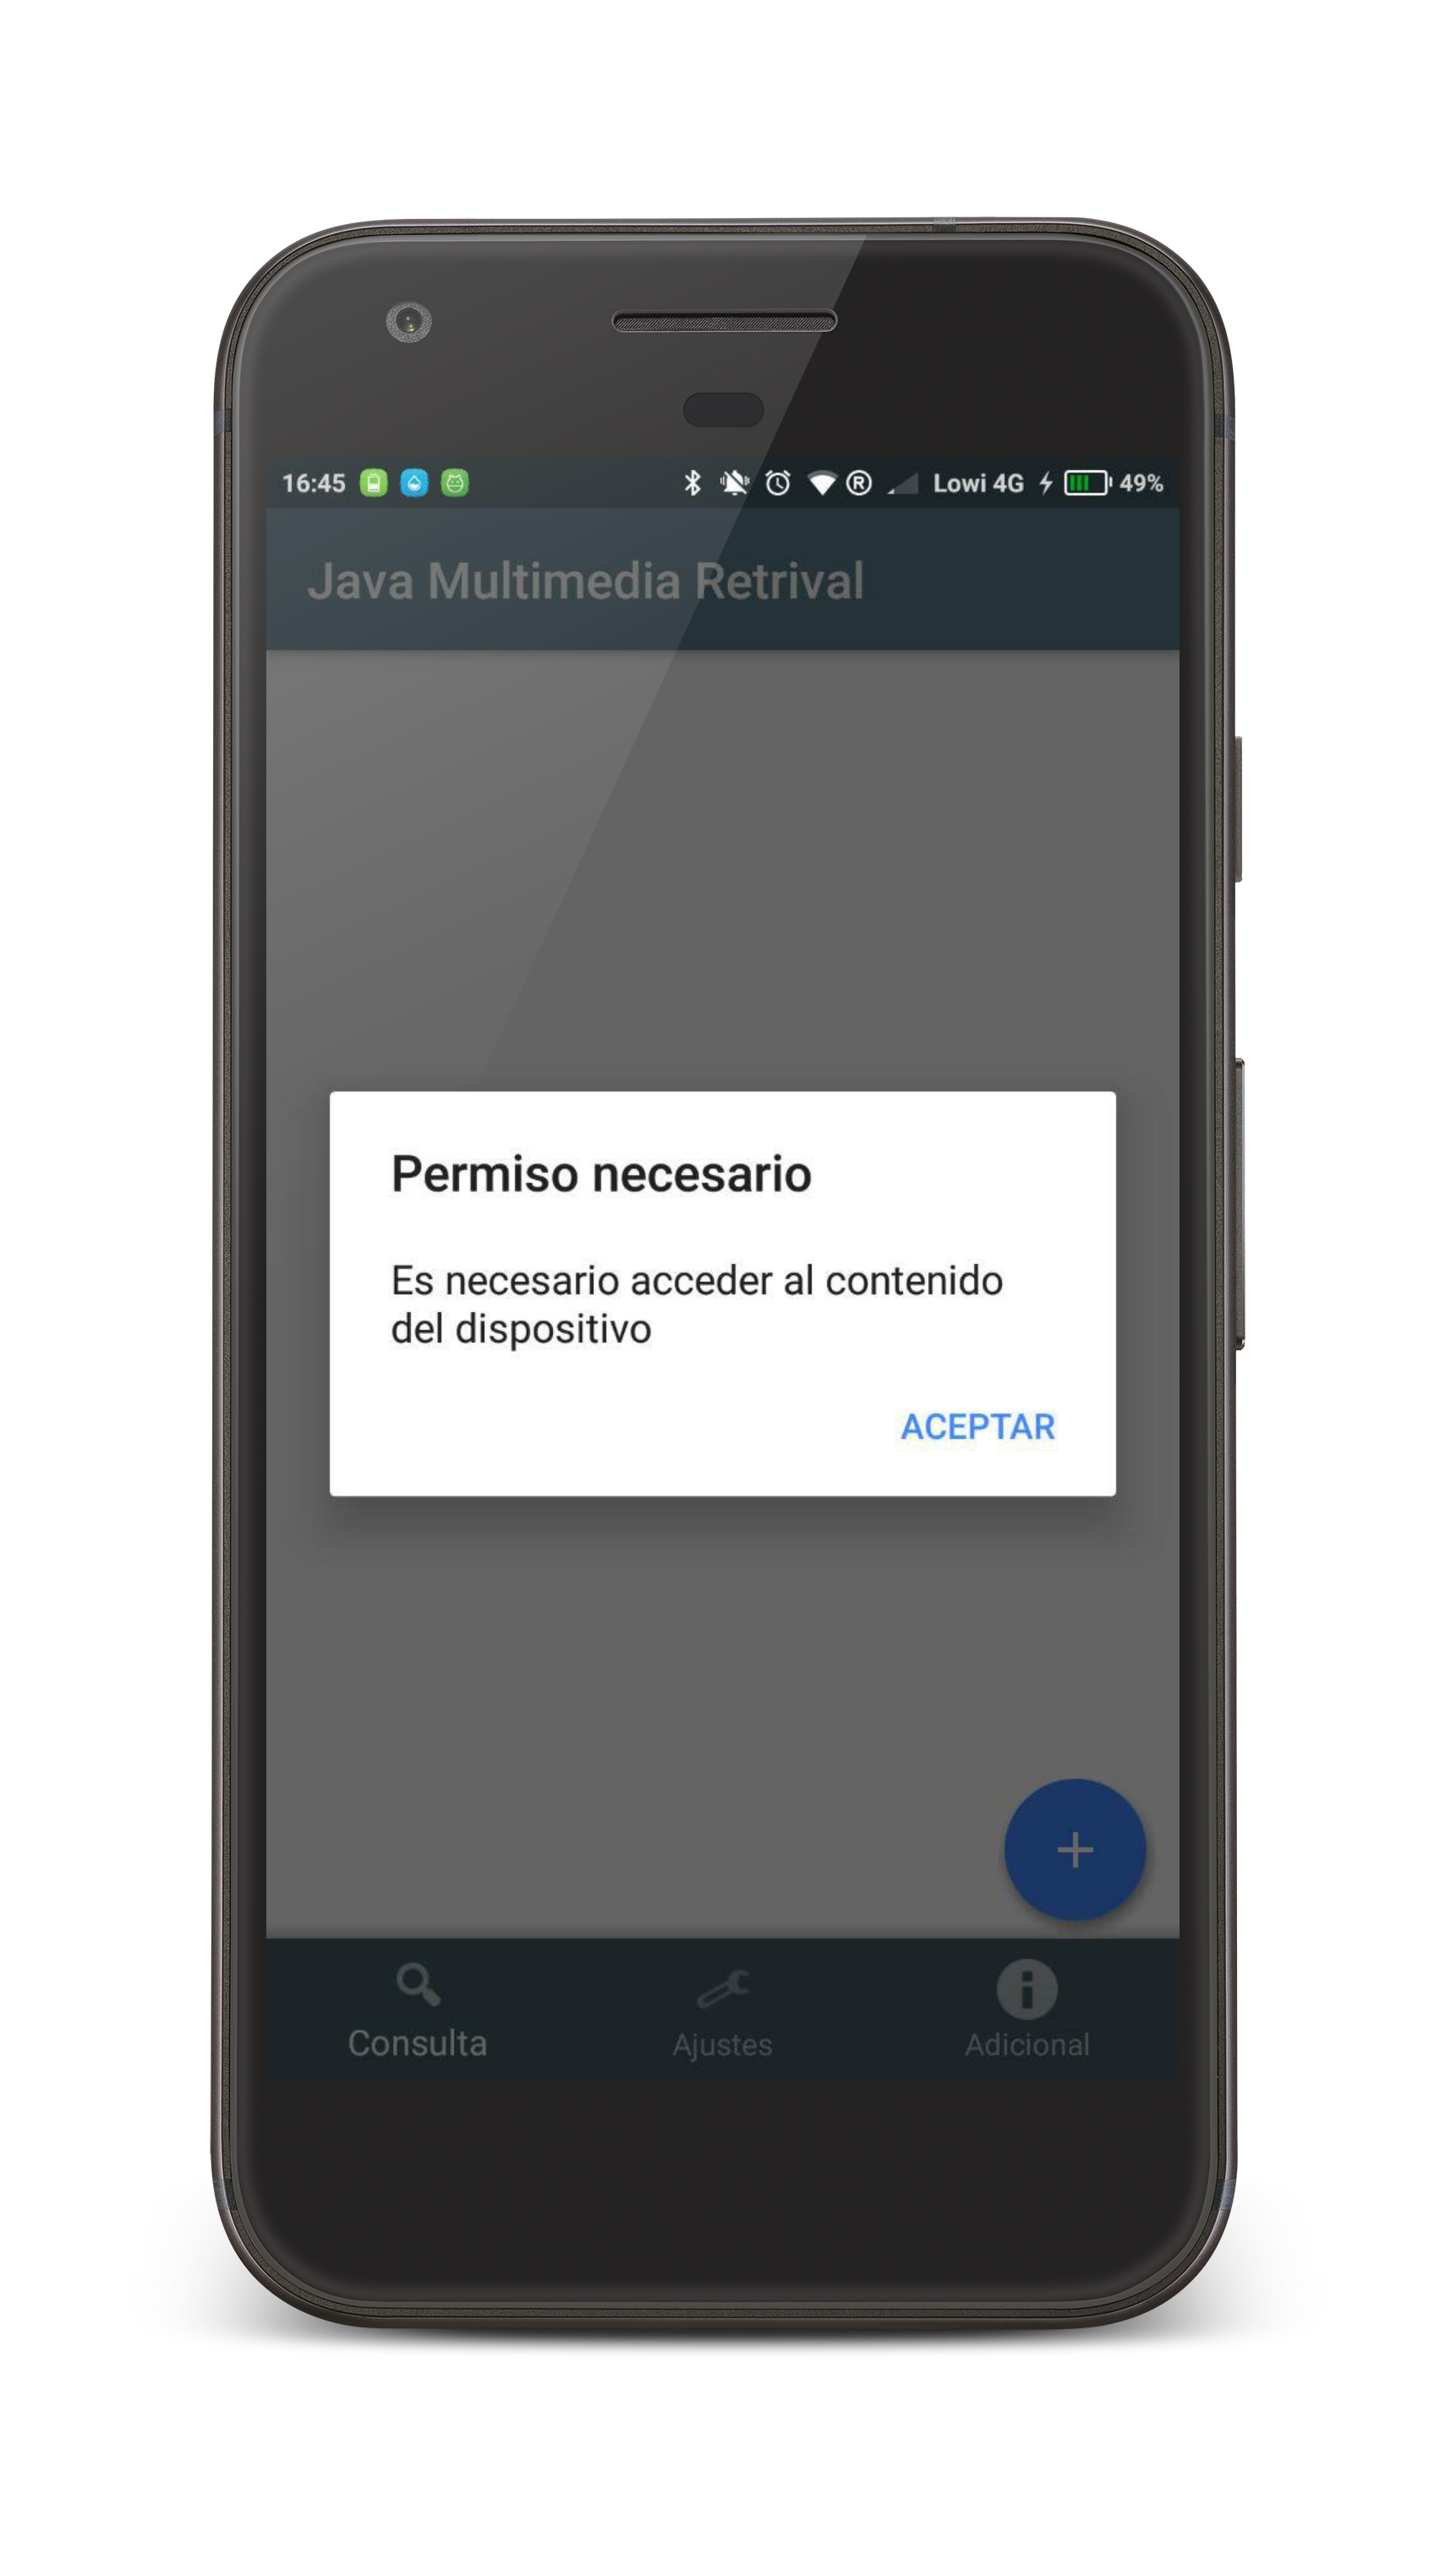
\includegraphics[scale=0.15]{imagenes/permisos2.png}  %el parámetro scale permite agrandar o achicar la imagen. En el nombre de archivo puede especificar directorios
\label{permisos2.png}
\caption{Permisos aplicación 2}
\end{figure}

\section{Navegación}

Para moverse a través de la aplicación, se dispone de un menú inferior con 3 elementos o ítems, cada uno representa una pantalla distinta. Por defecto la pantalla inicial es la correspondiente a la de consulta, ya que es el corazón de la aplicación.\\

Se pueden pulsar cada uno de los ítems para cambiar a su pantalla correspondiente. Cada pantalla tiene elementos propios y no son compartidos. Por ejemplo, el \textit{floating button} azul solo aparece en la pantalla de consulta.\\

\begin{figure}[H] %con el [H] le obligamos a situar aquí la figura
\centering
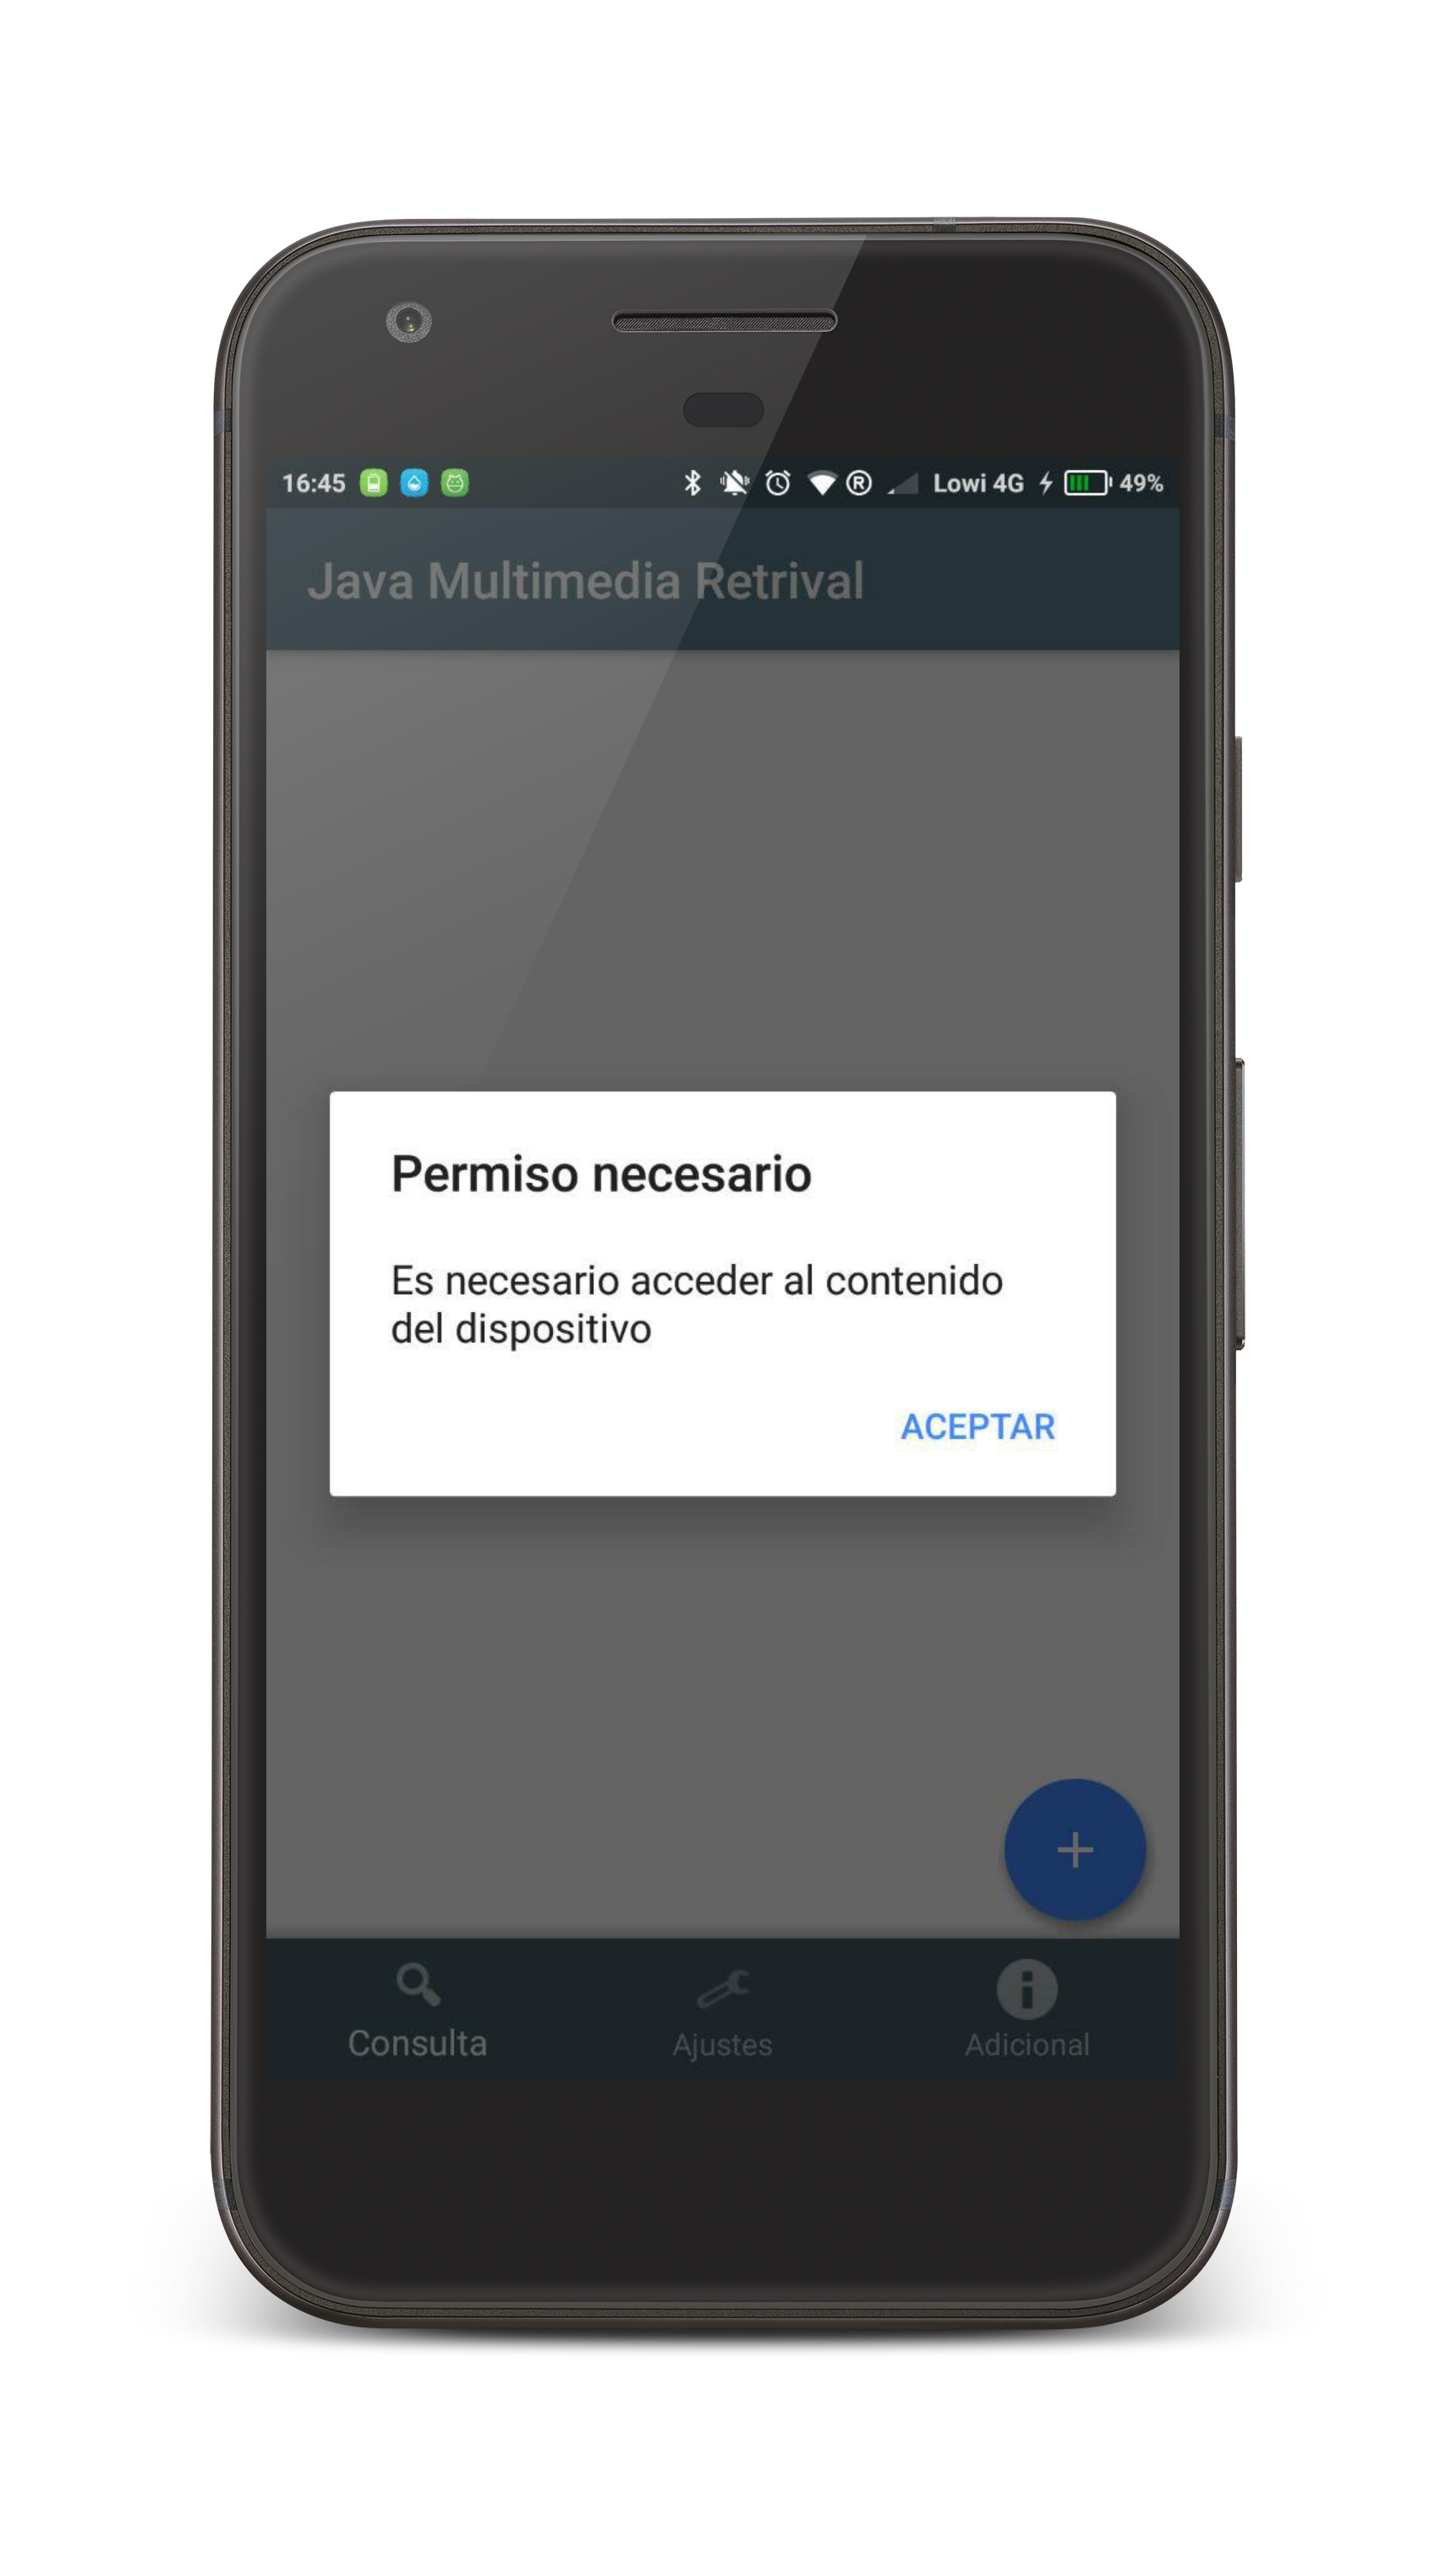
\includegraphics[scale=0.15]{imagenes/permisos2.png}  %el parámetro scale permite agrandar o achicar la imagen. En el nombre de archivo puede especificar directorios
\label{permisos2.png}
\caption{Ejemplo de navegación 1}
\end{figure}

\begin{figure}[H] %con el [H] le obligamos a situar aquí la figura
\centering
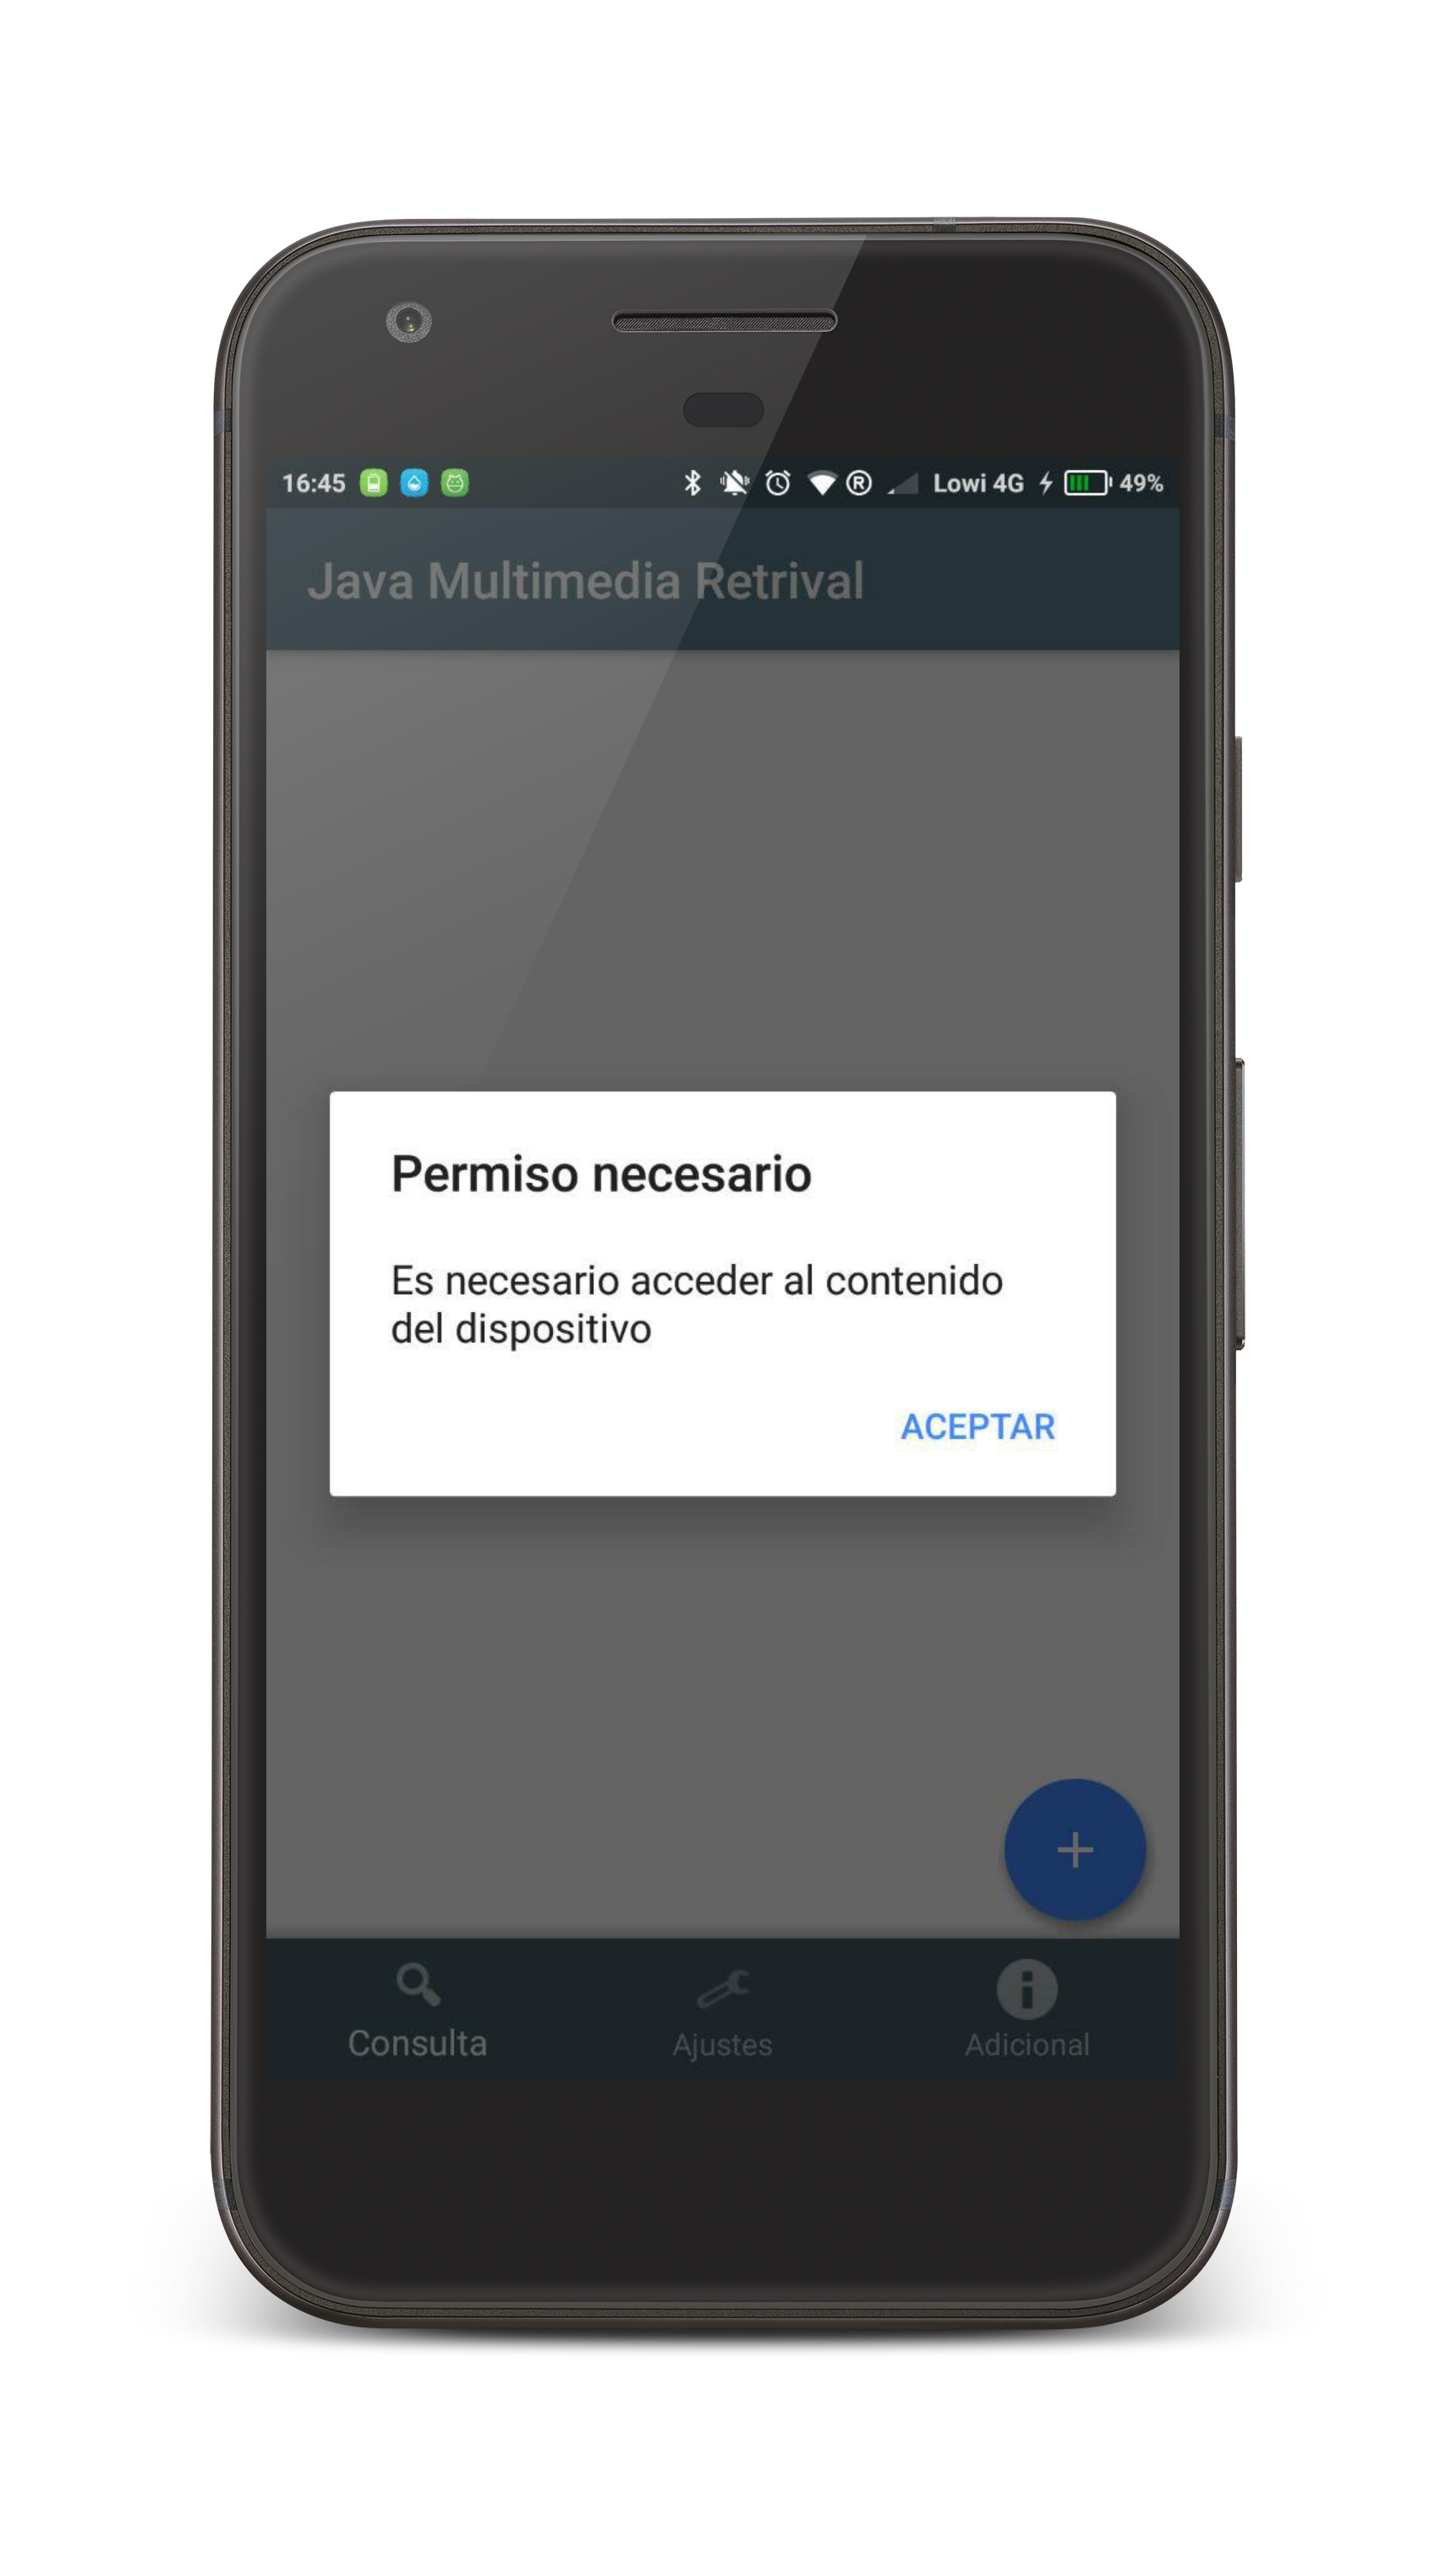
\includegraphics[scale=0.15]{imagenes/permisos2.png}  %el parámetro scale permite agrandar o achicar la imagen. En el nombre de archivo puede especificar directorios
\label{permisos2.png}
\caption{Permisos navegación 2}
\end{figure}

\section{Consulta}

Para realizar la consulta disponemos de dos opciones, elegir una imagen desde la cámara o desde la galería. Estas opciones aparecen al pulsar sobre el botón flotante. Una vez elegida una, se lanzará la cámara, pudiendo elegir la trasera o delantera, o la galería, mediante la cual podremos acceder a cualquier imagen del dispositivo. Cuando sea seleccionada, esta aparecerá en la parte superior de la aplicación.

\begin{figure}[H] %con el [H] le obligamos a situar aquí la figura
\centering
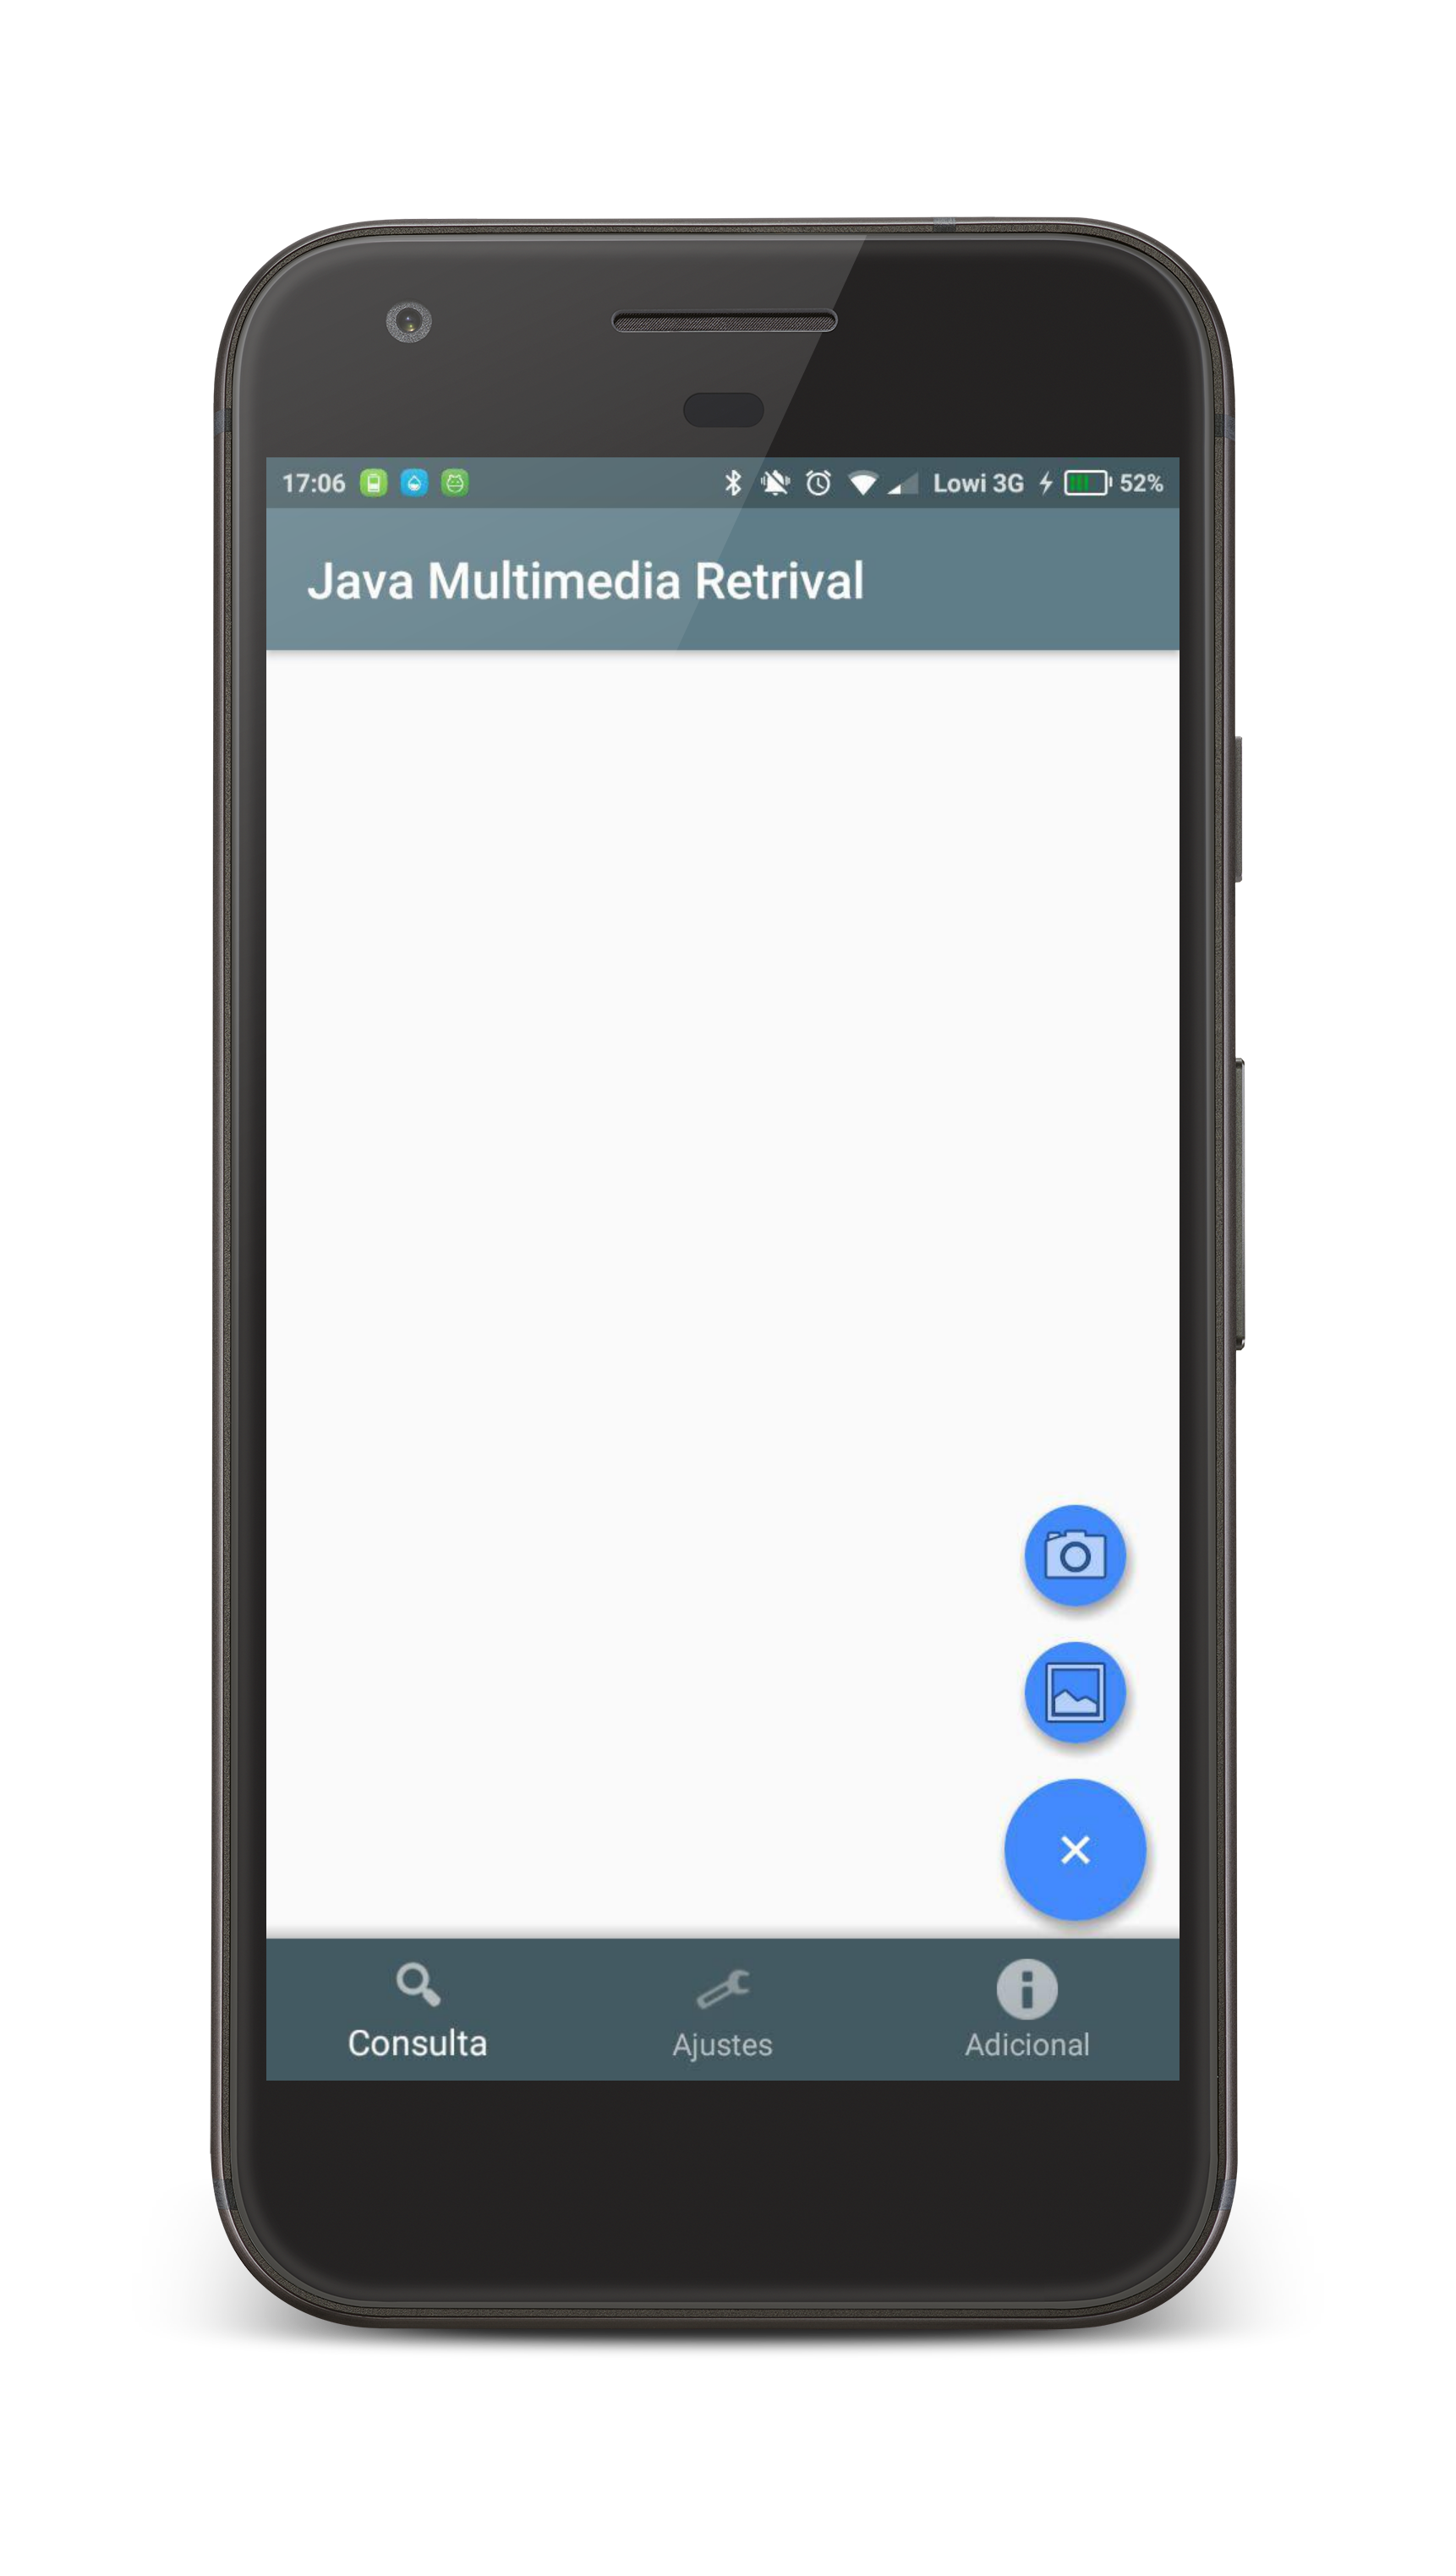
\includegraphics[scale=0.15]{imagenes/hacerconsulta.png}  %el parámetro scale permite agrandar o achicar la imagen. En el nombre de archivo puede especificar directorios
\label{hacerconsulta.png}
\caption{Realizar consulta}
\end{figure}

\section{Ajustes}

En este apartado vamos a hablar de los ajustes que puede realizar el usuario sobre las consultas.\\

\begin{figure}[H] %con el [H] le obligamos a situar aquí la figura
\centering
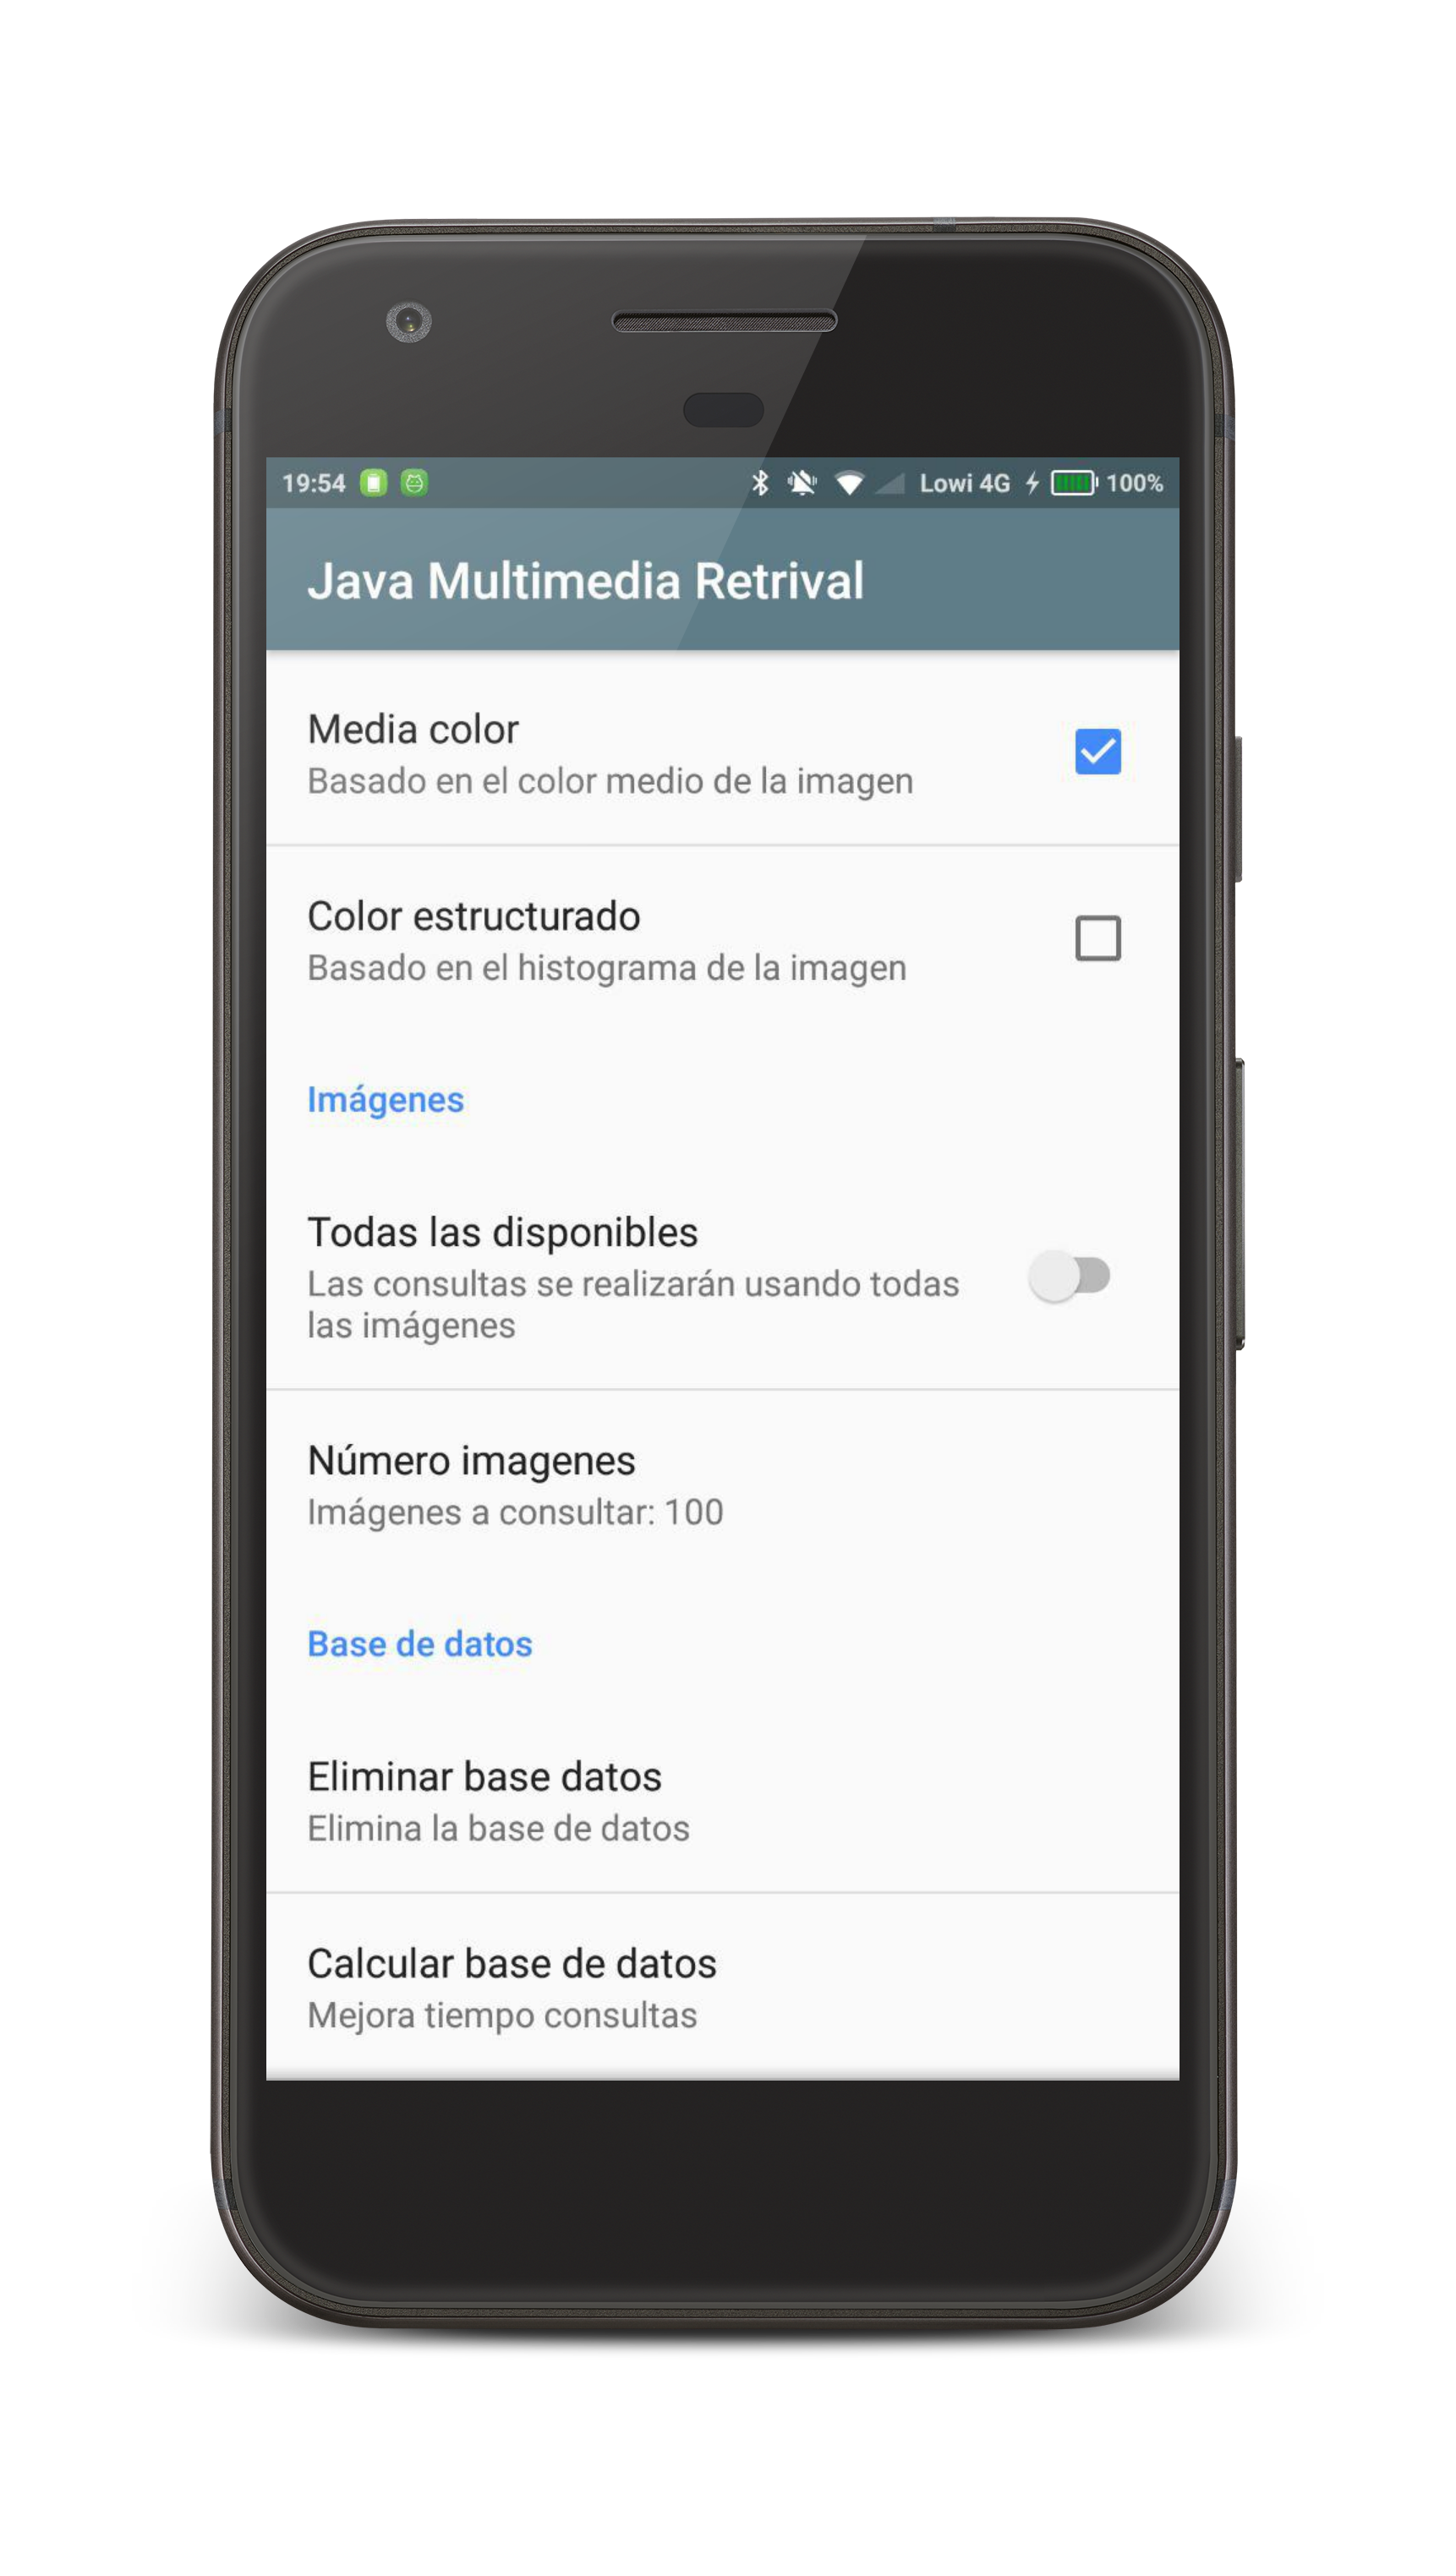
\includegraphics[scale=0.15]{imagenes/ajustes.png}  %el parámetro scale permite agrandar o achicar la imagen. En el nombre de archivo puede especificar directorios
\label{ajustes.png}
\caption{Pantalla ajustes}
\end{figure}

Podríamos hablar de tres secciones:

\subsection{Descriptores}

Aquí podemos encontrar los descriptores de los que dispone la aplicación. El usuario puede elegir uno libremente, pero solo un descriptor puede ser elegido a la vez.

\begin{figure}[H] %con el [H] le obligamos a situar aquí la figura
\centering
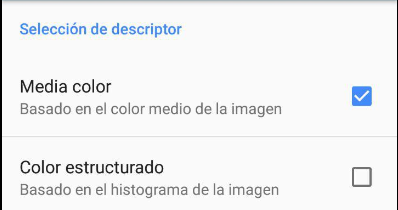
\includegraphics[scale=0.5]{imagenes/ajustesdescriptor.png}  %el parámetro scale permite agrandar o achicar la imagen. En el nombre de archivo puede especificar directorios
\label{ajustesdescriptor.png}
\caption{Pantalla ajustes. Sección descriptores}
\end{figure}

\subsection{Imágenes}

En este apartado el usuario puede elegir el número de imágenes totales sobre las cuales quiere realizar la consulta. Tiene dos opciones, introducir dicho valor manualmente o seleccionar todas las del dispositivo. Este valor también se usa en el caso de querer calcular la base de datos, cosa que veremos a continuación.

\begin{figure}[H] %con el [H] le obligamos a situar aquí la figura
\centering
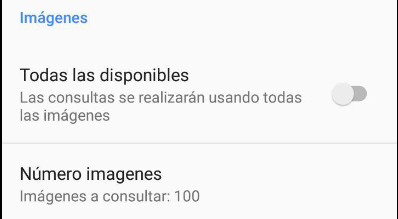
\includegraphics[scale=0.5]{imagenes/ajustesimagenes.png}  %el parámetro scale permite agrandar o achicar la imagen. En el nombre de archivo puede especificar directorios
\label{ajustesimagenes.png}
\caption{Pantalla ajustes. Sección imágenes}
\end{figure}

\subsection{Base de datos}

Aquí el usuario puede precalcular la base de datos, de esta manera al realizar la consulta no se calcularán nada, simplemente se obtendrán los valores de la base de datos. Este precálculo se realiza para todos los descriptores del sistema.\\

Por otro lado, puede borrar la base de datos si así lo desea. Realizando se calcularán los valores de la base de datos durante la consulta.

\begin{figure}[H] %con el [H] le obligamos a situar aquí la figura
\centering
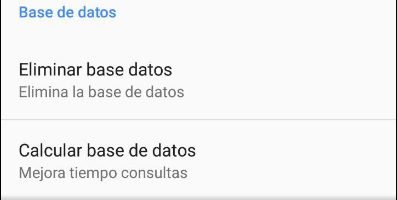
\includegraphics[scale=0.5]{imagenes/ajustesbd.png}  %el parámetro scale permite agrandar o achicar la imagen. En el nombre de archivo puede especificar directorios
\label{ajustesbd.png}
\caption{Pantalla ajustes. Sección base de datos}
\end{figure}

\section{Adicional}

En esta sección el usuario puede encontrar información relacionada con el proyecto, así como sobre su desarrollador. Al pulsar en cualquier opción esta le llevará a su correspondiente página web con una mayor cantidad de información.\\

Debido a que este tipo de sistema, \textit{CBIR}, no es muy conocido por los usuarios, al igual que los descriptores, se proporciona una serie de enlaces con información básica sobre ellos, en caso de que el usuario quiera aprender más o sienta curiosidad sobre el tema.

\begin{figure}[H] %con el [H] le obligamos a situar aquí la figura
\centering
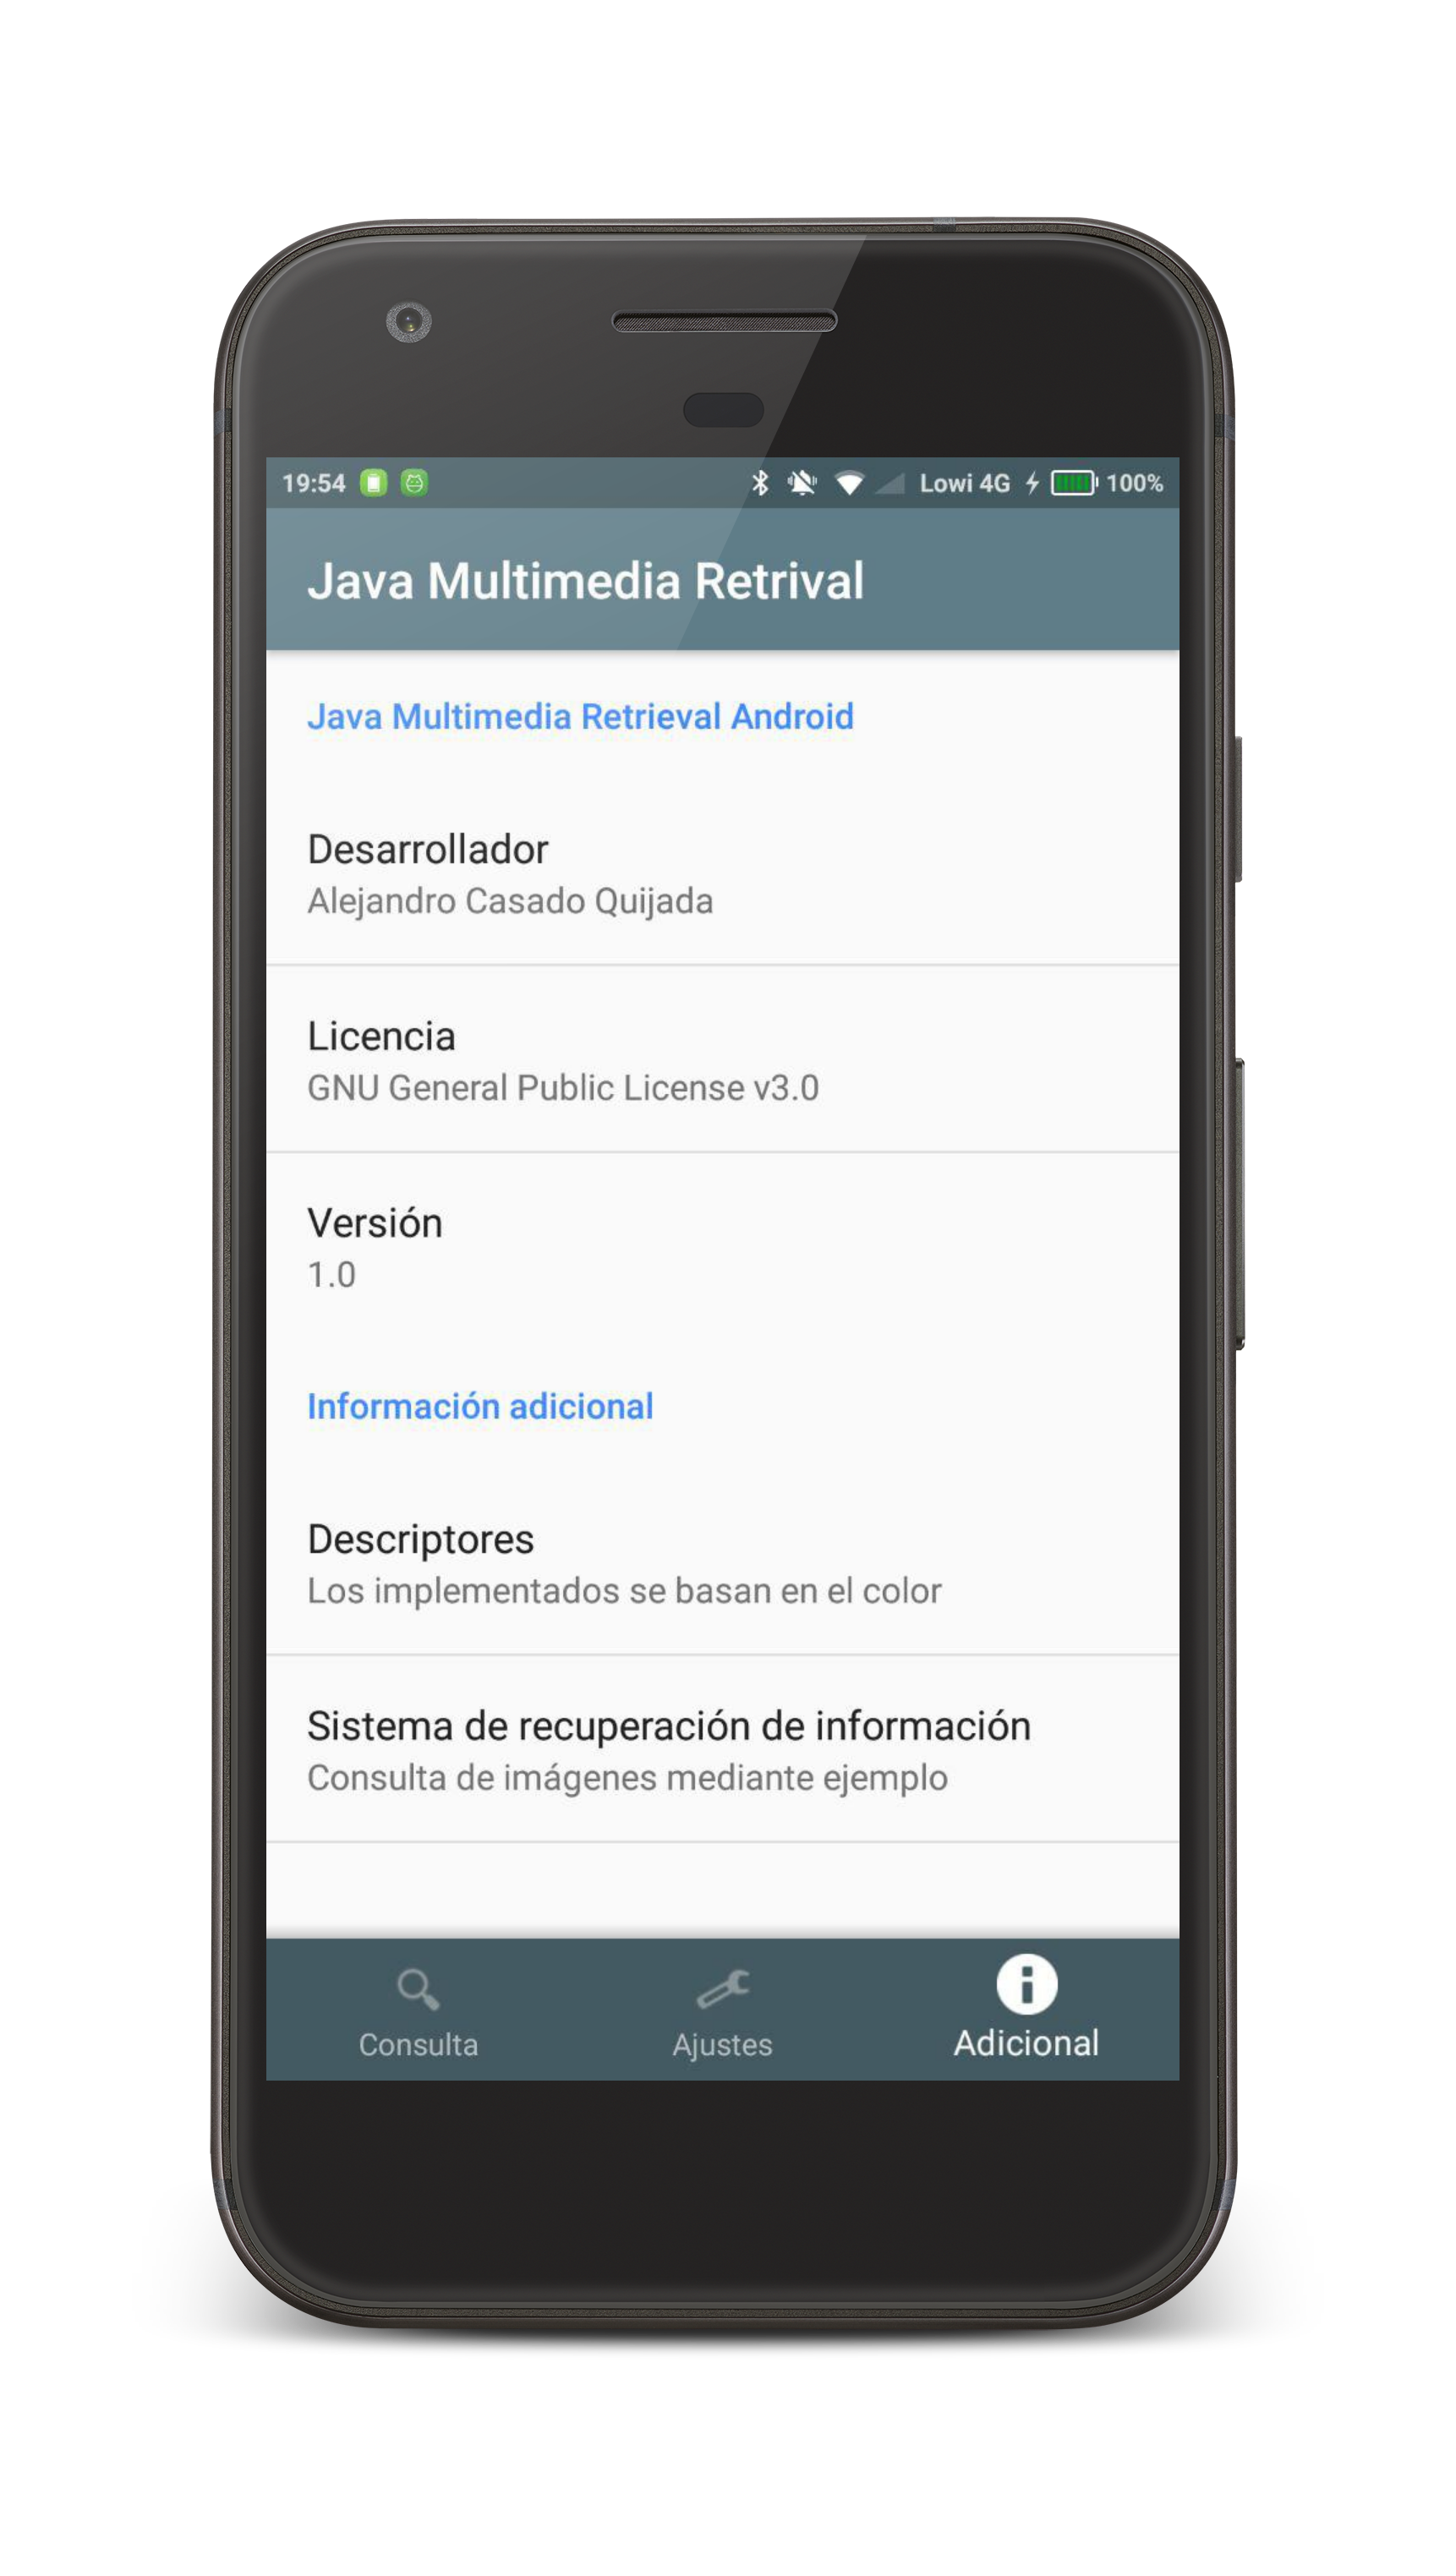
\includegraphics[scale=0.15]{imagenes/adicional.png}  %el parámetro scale permite agrandar o achicar la imagen. En el nombre de archivo puede especificar directorios
\label{adicional.png}
\caption{Pantalla adicional}
\end{figure}









%\input{apendices/licencia/licencia}
%%\input{apendices/paper/paper}
%\input{glosario/entradas_glosario}
% \addcontentsline{toc}{chapter}{Glosario}
% \printglossary
%\chapter*{}
\thispagestyle{empty}

\end{document}
